% *****************************************************************************
%     sections/chapter2.tex
%
% Last edit: 23/04
% *****************************************************************************

\chapter{Bayesian inference of neutron star observables}

This chapter deals with the determination of NS observables within a Bayesian 
framework.

Pulsars were identified to rotating NS which produce pulsed emission, soon 
after their chance discovery in 1967 by Jocelyn Bell~\cite{Hewish1968}. Five
decades later, we have now observed about 2000 of them, and numerous techniques
have been developed to measure their characteristic observables. For instance, 
precise measurements of NS masses can be performed using the relativistic 
Shapiro delay effect~\cite{Demorest2010,Antoniadis2013,Cromartie2020}, the
ambitious NICER program {is giving more and more constraining information 
  on the NS radii
\cite{Bogdanov2019a,Bogdanov2019b,Miller2019,Raaijmakers2019,Riley2019}}, and 
the first detection of GW from the coalescence of two NS, the GW170817 event, 
has provided a
constraint on the tidal deformability of NS~\cite{GWtidal,GW1,GW2}. All those
experimental data can be used to better constrain the nuclear EoS. 
Reciprocally, there has been a lot of efforts invested recently in the 
development of ab initio calculations, particularly based on the chiral 
EFT~\cite{Drischler2016} with the aim of providing new 
constraints on the low-density EoS, which can
ultimately be translated into theoretical constraints on NS
observables~\cite{Carreau2019cc,Carreau2019moi}.
In this context, the Bayesian framework is particularly appealing for making 
realistic predictions for NS observables. It allows to update our prior beliefs 
on the EoS parameters with the constraints arising from the multiple sources 
mentioned above.

The plan of the chapter is as follows. In Section~\ref{sec:tov}, global
properties and crustal observables are calculated for several characteristic 
EoS by solving the equations of hydrostatic equilibrium in general relativity.
The connection between the crust moment of inertia and the glitch phenomenon is
explained. The EoS parameters are determined within a 
Bayesian framework in~\ref{sec:bayes}, given the present day constraints on
nuclear physics, NS observables, and physical requirements. In particular,
correlations among the empirical parameters are explored. General predictions
for NS observables are proposed in~\ref{sec:general}, using the joint posterior
distribution of EoS parameters. We confront our predictions with different 
constraints inferred from the GW170817 event. The CC transition density and
pressure as well as the fractional crust moment of inertia are evaluated. The
full crustal origin of Vela pulsar glitches is discussed. Finally, conclusions 
are given in Section~\ref{sec:conclu2}.

\minitoc\newpage

\section{From the equation of state to neutron star observables}\label{sec:tov}

The stellar EoS, the determination of which was studied thoroughly in Chapter 
1, is the fundamental ingredient to build NS models. It enters into the 
basic equation for calculating macroscopic observables relevant to NS, the 
so-called Tolman-Oppenheimer-Volkoff (TOV) equation, which describes the 
hydrostatic equilibrium for a spherically symmetric nonrotating star in the 
framework of general relativity~\cite{Tolman1939,Oppenheimer1939}.

This section deals with the estimation of NS observables for several 
popular EoS calculated within the metamodeling technique introduced in 
Chapter 1. In~\ref{subsec:masses}, we first solve the hydrostatic 
equilibrium equations so as to determine the mass-radius relation. The 
thickness and mass of the crust are also evaluated. The calculation of the NS 
moment of inertia in the slow rotation approximation is performed 
in~\ref{subsec:moi}. In particular, we show how the fractional crust moment 
of inertia is connected to the 
observation of pulsar glitches. In~\ref{subsec:tidal}, we finally compute the 
tidal deformability, which describes how much the NS is deformed by tidal 
forces, arising, for instance, in the final approach phase of two merging NS.

\subsection{Masses and radii}\label{subsec:masses}

% observations
% From the observational point of view, it is easier for astronomers to measure 
% the mass of a NS belonging to a binary system. There are several types of
% binaries: x-ray binaries, double NS binaries, radio pulsar--white dwarf 
% binaries, and radio pulsar--nondegenerate star binaries. Depending on the type 
% of binary, different techniques are used to infer the NS 
% mass~\cite{Haensel2007}.
% % Shapiro delay effect - MSP
% For example, in a pulsar binary system, various phenomena, such as the 
% relativistic Shapiro delay~\cite{Shapiro1964}, can be exploited for the aim of
% mass measurement via pulsar 
% timing, which consists in the regular monitoring of the rotation of a pulsar 
% over long periods (years to decades). The relativistic Shapiro delay is a 
% phenomenon from which precise masses for both a millisecond pulsar and its 
% companion can be inferred~\cite{Demorest2010,Cromartie2020}. Let us notice 
% however that it is only observed in a small subset of high-precision, highly 
% inclined binary pulsar systems. 
% % Measuring NS radii is less straightforward
% Measuring NS radii with high precision is a more challenging task, and reliable
% constraints have started to be available only in a very recent 
% past \cite{Bogdanov2019a,Bogdanov2019b,Miller2019,Raaijmakers2019,Riley2019}. 
% This observable can be extracted from the analysis of thermal emission from 
% neutron star surfaces -- even if complications in the interpretation of the data
% arise due to the nonuniformity of the temperature over the surface (hot
% spots) \cite{Bogdanov2019a,Bogdanov2019b,Miller2019,Raaijmakers2019,Riley2019}
% --, or x-ray emission from accreting neutron stars in binaries.

In the following, we turn to the theoretical prediction of NS masses and radii. 
The hydrostatic equilibrium equations in general relativity are first solved in 
order to represent the mass-radius relation for several popular EoS, which are
then confronted to NS mass measurements. The estimation of the crustal 
thickness and mass is discussed later in~\ref{subsubsec:crustthickmass}.

\subsubsection{Mass-radius relation}

% hydrostatic equilibrium in GR
Theoretically, the NS masses and radii correspond to the 
solution of the hydrostatic equilibrium equations, which are, in general 
relativity for spherical and nonrotating 
stars, given by~\cite{Tolman1939,Oppenheimer1939}
%
\begin{eqnarray}
  \frac{dP}{dr} &=& -\frac{G\rho_B m}{r^2}\left(1 + \frac{P}{\rho_B
  c^2}\right)\left(1+\frac{4\pi
  Pr^3}{mc^2}\right)\left(1-\frac{2Gm}{rc^2}\right)^{-1},\label{eq:tov}\\
      \frac{dm}{dr} &=& 4\pi r^2\rho_B,\label{eq:massbal}\\
  \frac{d\Phi}{dr} &=& -\frac{1}{\rho_B
    c^2}\frac{dP}{dr}\left(1+\frac{P}{\rho_B
  c^2}\right)^{-1}\label{eq:metric},
\end{eqnarray}
%
where $G$ is the gravitational constant, $P$ the pressure, $\rho_B c^2$ the
energy density, and $m(r)$ the is the gravitational mass inside the sphere of
radius $r$, defined within the Schwarzschild metric $ds^2 = c^2dt^2e^{2\Phi} 
- e^{2\lambda}dr^2 - r^2(d\theta^2 + \sin^2\theta d\phi^2)$. The function 
$\Phi(r)$ corresponds to the gravitational potential, and $\lambda(r)$ is 
related to the enclosed mass $m(r)$ through
%
\begin{equation}
  e^{-\lambda} = \sqrt{1-\frac{2Gm}{rc^2}}.
\end{equation}
%
% description of the equations
Eq.~(\ref{eq:tov}) is called the TOV equation 
of hydrostatic equilibrium. The integration of Eq.~(\ref{eq:massbal}) from
$r=0$ to the boundary $r=R$, $R$ being the NS radius, gives the total
gravitational mass $M=m(R)$ of the star. Eq.~(\ref{eq:metric}) is a 
relativistic equation for the metric function $\Phi(r)$. This equation will be
needed for the computation of the moment of inertia in~\ref{subsec:moi}. Here, 
we focus on solving Eqs.~(\ref{eq:tov}) and 
(\ref{eq:massbal}), which gives the profiles $P(r)$, $\rho_B(r)$, and $m(r)$ 
for a given EoS, $P(\rho_B)$, the determination of which was discussed in 
detail in Chapter 1.

% explain numerical method for a central density nc (CGS, Euler method, 
%   lagrangian interpolation)
In view of solving the hydrostatic equilibrium equations for a given tabulated 
EoS, one first has to choose an arbitrary value for the central density 
$\rho_{B,c}$ and 
interpolate the central pressure $P_c = P(\rho_{B,c})$, corresponding to $r=0$, 
with the associated boundary condition $m(r=0) = 0$. Then, using a Runge-Kutta 
method, we integrate up to $r=R$, defined as $P(r=R) = 0$ (our numerical 
condition is $P < 5\times 10^{-4}$ MeV/fm$^{3}$, which is a sufficiently low 
value of the pressure to get convergent values for the total mass). At each new 
step of pressure, one has to interpolate 
the mass density $\rho_B$ in the table. In the end, for a given value of 
central density $\rho_{B,c}$, one obtains the profiles $P(r)$, $\rho_B(r)$, 
and $m(r)$, and therefore a value for the NS mass $M$ and radius $R$. The 
typical canonical value of the NS mass is $M=1.4M_\odot$, with a corresponding
radius $R=10-14$ km~\cite{Haensel2007}. 
% The problem is that the central density inside a NS is not known... thats why 
%   we are interested in the Mass radius relation
In fact, the central density inside a specific NS is not known, and is expected
to range from $\approx 4.6\times 10^{14}$ g/cm$^3$ to $\approx 4\times 10^{15}$
g/cm$^3$. For this reason, we are rather interested in the mass-radius 
relation, which can be obtained by calculating $M$ and $R$, following the 
numerical method previously explained, for that range of central mass 
densities\footnote{Let us recall that one has to redefine the high-order 
  parameters $Q_{sat(sym)}$ and $Z_{sat(sym)}$ in order to reproduce existing 
  functionals at densities greater than $2n_{sat}$ with the metamodeling 
  technique. This corresponds to the ELFd technique introduced 
in \cite{Margueron2018a}, see~\ref{subsec:icore}.}.

\begin{table}[!t]
\begin{center}
\begin{tabular}{cccccc} 
  \toprule
  \toprule
  Parameter & Unit & $N$ & BSk14 & PKDD & TM1\\
  \midrule
  $E_{sat}$ & MeV & 0         & -15.85 & -16.27  & -16.26 \\
  $n_{sat}$ & fm$^{-3}$ & 1   & 0.1586 &  0.1495 & 0.1450 \\ 
  $K_{sat}$ & MeV & 2         & 239    &  261    & 281    \\ 
  $Q_{sat}$ & MeV & 3         & -359   &  -119   & -285   \\ 
  $Z_{sat}$ & MeV & 4         & 1435   &  4213   & 2014   \\ 
  $E_{sym}$ & MeV & 0         & 30.00  &  31.19  & 36.94  \\
  $L_{sym}$ & MeV & 1         & 43.9   &  79.5   & 111.0  \\
  $K_{sym}$ & MeV & 2         & -152   &  -50    & 34     \\
  $Q_{sym}$ & MeV & 3         & 389    &  -28    & -67    \\
  $Z_{sym}$ & MeV & 4         & -2191  &  -1315  & -1546  \\
  $m_{sat}^*/m$ & &           & 0.80   &  0.65   & 0.71   \\
  $\Delta m_{sat}^*/m$ & &    & 0.03   &  -0.08  & -0.09  \\
  \bottomrule
  \bottomrule
\end{tabular}
\end{center}
\caption[Empirical parameters for BSk14, PKDD, and TM1]{Value of each of the 
  empirical parameters, associated unit, and derivative order $N$ for BSk14 
  \cite{Goriely2007}, PKDD \cite{Long2004}, and TM1~\cite{Sumiyoshi1995} 
functionals.}\label{table:newemppar}
\end{table}

\begin{figure}[!t]
\begin{center}
  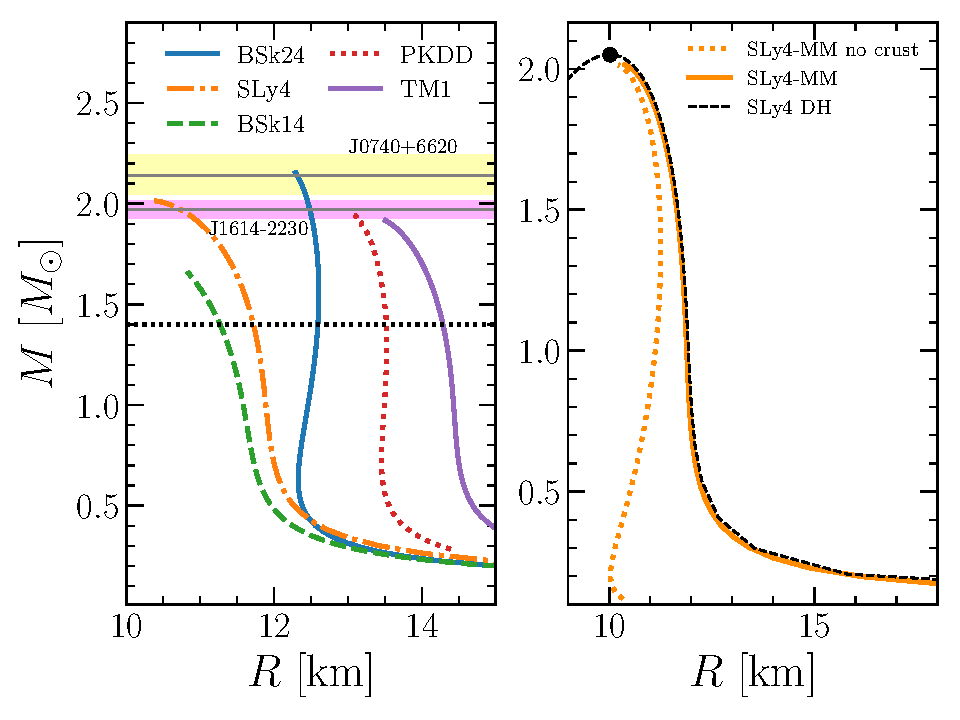
\includegraphics[width=0.9\linewidth]{figures/mr_popular.pdf}
\end{center}
\caption[Mass-radius relation for several popular equations of state]{Left: 
  Mass-radius relation for several popular EoS calculated
  with the metamodeling technique. The black dotted line marks the NS 
canonical mass, that is $1.4M_\odot$. The magenta band represents the measured 
mass of PSR J0348+0432, $(2.01 \pm 0.04)M_\odot$ \cite{Antoniadis2013}, and the 
yellow band that of PSR J0740+6620, $2.14_{-0.09}^{+0.10}M_\odot$ ($68.3\%$ 
credibility interval) \cite{Cromartie2020}.
Right: Mass-radius relation for the DH EoS for SLy4 functional (black dashed
line), and the SLy4 EoS calculated with the metamodeling technique (solid
orange line). The black circle indicates the maximum 
mass.}\label{fig:mr_popular}
\end{figure}
 
The left panel of Fig.~\ref{fig:mr_popular} shows the mass-radius relation for 
several popular EoS based on Skyrme-type functionals BSk24, SLy4, and BSk14, 
and relativistic models PKDD and TM1, calculated within the metamodeling 
technique. A strong model dependence is observed, with radii of canonical NS 
ranging from $R_{1.4}=11.5$ km for BSk14\footnote{The BSk14 parametrization is
an old representative of the BSk functionals. More modern versions of the BSk
family are employed elsewhere in this thesis. Even if it does not belong to the
most up-to-date functionals, it gives a good illustration of the prediction of
a very soft EoS.} to $R_{1.4}=14.5$ km for TM1. More
specifically, it is seen that a stiffer density dependence of the symmetry
energy leads to larger radii. Indeed, a positive correlation between $R_{1.4}$
and $L_{sym}$ has been often highlighted in the literature
\cite{Alam2016,Ji2019,Hu2020}. However, to pin down which is the more
influential parameter that determines the NS radius, a simple comparison
between models is not enough, and a full statistical analysis is needed. Such
analysis is presented in Section~\ref{sec:general}. The value of the empirical 
parameters associated to BSk14, TM1, and PKDD are reported in 
Table~\ref{table:newemppar}, 
whereas those of BSk24 and SLy4 can be found in Table~\ref{table:emp_params}.
The bands correspond to the measured masses of the two most massive
pulsars observed to the present day. The mass of PSR J0348+0432 was precisely 
estimated to $(2.01\pm 0.04)M_\odot$~\cite{Antoniadis2013}, and the very recent
relativistic Shapiro delay measurements of PSR J0740+6620 led to 
$2.14_{-0.09}^{0.10}M_\odot$ ($68.3\%$ credibility
interval)~\cite{Cromartie2020}. Naturally, if an
EoS cannot insure such high masses, it should not be considered as reliable, 
in particular at high density, since the maximum mass is determined by the 
stellar core EoS. In particular, it is seen that the maximum mass corresponding
to the BSk14 functional, $1.8M_\odot$, is lower than the measured mass
of PSR J0348+0432. Also, while the SLy4 EoS satisfy this constraint, the maximum 
mass for this EoS, $2.05M_\odot$, is lower than that of PSR J0740+6620. This 
outlines the fact that measuring the mass of pulsars is important, because it 
provides a strong constraint on the stellar matter EoS. Similarly, the NICER
telescope is expected to provide, for years to come, a constraint on the NS
radii with a precision of $5\%$. Ultimately, in the ideal case where one could 
accurately measure the mass and radius of one neutron star, it would be 
possible to determine the EoS by positioning the point in the $M-R$ diagram.

The mass-radius relation for the SLy4 EoS is represented in the right panel of
Fig.~\ref{fig:mr_popular}. The solid orange line corresponds to $M(R)$ for the 
SLy4 EoS calculated within the metamodeling technique, and the dashed 
black line is the calculation for the same SLy4 functional
from~\cite{Douchin2001}. A perfect agreement is observed between the two 
curves, reflecting the small discrepancy between the EoS, already illustrated 
in Fig.~\ref{fig:unified}. 
The dotted orange line shows the mass-radius relation for the SLy4 EoS without
considering the clustering of matter at low density, that is assuming that the
NS star interior consists of homogeneous $npe\mu$ matter at all densities. In 
that case, for a canonical NS, we find $R_{1.4} = 11.1$ km, which is almost $1$ 
km lower with respect to the result with a crust EoS. 
Moreover, this difference is found to be larger with decreasing mass. 
This shows that the crust EoS is essential to properly predict NS
radii~\cite{Perot2020}. 
However, we can see that the NS maximum mass is entirely determined by the 
stellar core EoS.
The black point marks the maximum mass for the SLy4 EoS, $M_{max} = 
2.05M_\odot$. Let us notice that the branch left to the point is unstable, 
because from this point the mass decreases with increasing central density.

\subsubsection{Crust thickness and mass}\label{subsubsec:crustthickmass}
% crust thickness and mass
As explained in Chapter 1, a precise estimation of the CC transition point is
required as far as crustal properties are concerned. In particular, the
transition pressure $P_t$ is essential for the determination of the thickness 
and mass of the crust, given respectively by $l_{crust}=R-R_{core}$ and
$M_{crust}=M-M_{core}$, with $R_{core}$ ($M_{core}$) the radius
(mass) of the stellar core. Indeed, in order to calculate the core radius and
mass, which are involved in the calculation of the crustal observables, one has 
to integrate the hydrostatic equilibrium equations, Eqs.~(\ref{eq:tov}) and 
(\ref{eq:massbal}), from $r=0$ to $r=R_{core}$, defined as $P(r=R_{core})=P_t$.

\begin{figure}[!t]
\begin{center}
  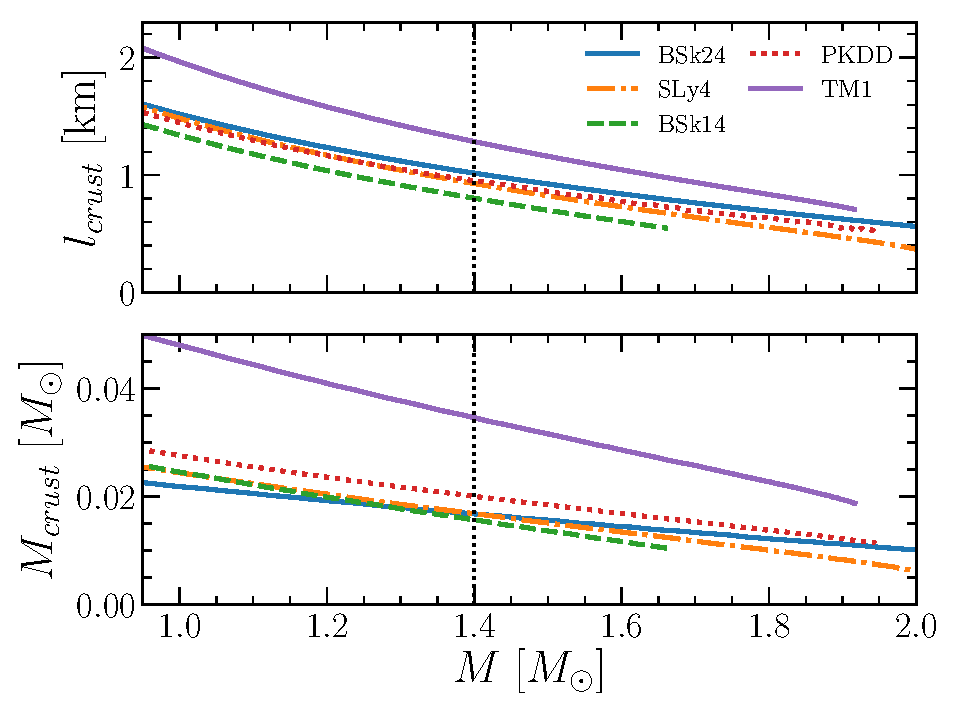
\includegraphics[width=0.9\linewidth]{figures/crustmassthick.pdf}
\end{center}
\caption[Crust thickness and mass versus neutron star mass for several 
popular equations of state]{Crust 
  thickness $l_{crust}$ (upper panel) and mass $M_{crust}$ (lower panel) as a 
  function of the NS mass $M$ for several popular EoS calculated within the 
  metamodeling technique. The black dotted line marks the NS canonical mass, 
  that is $1.4M_\odot$.}\label{fig:crustmassthick}
\end{figure}

Fig.~\ref{fig:crustmassthick} shows the variation with NS mass of crust 
thickness $l_{crust}$ and mass $M_{crust}$ for the same EoS as in 
Fig.~\ref{fig:mr_popular}. As explained in~\ref{subsec:icore}, for each
functional, when we integrate the TOV equation, the high-order empirical 
parameters are redefined such as to optimize the reproduction of the
high density EoS. 
However, the transition pressure is calculated using the values of 
$Q_{sat(sym)}$ and $Z_{sat(sym)}$ derived from the Taylor expansion at 
saturation. The reason is that, as showed in Fig.~\ref{fig:sly4_nt}, the 
determination of CC transition point is sensitive to orders $N>2$, and the
Taylor expansion around saturation is reliable in the subsaturation regime. 
We find the interesting result that the crust is thicker for low-mass neutron 
stars, and that $M_{crust}$ drops continuously with 
increasing NS mass. At $M=1.4M_\odot$ (black dotted line), we 
observe that the crust is $\approx 1$ km thick, and that the crust mass is 
approximately $0.02-0.04M_\odot$, which is $(1.5-3)\%$ of the total mass. Once
again, a model dependence is observed. Nonetheless, the correlation of the 
crust thickness with the stiffness of the EoS is not clear. 
In Fig.~\ref{fig:mr_popular}, we have seen that the radius of the 
star is positively correlated with the stiffness of the density dependence of
the symmetry energy. In fact, the same is true for the 
core radius, explaining why the correlations are less evident in the crust 
thickness $l_{crust} = R - R_{core}$.

\subsection{Moment of inertia within the slow rotation
approximation}\label{subsec:moi}

We now turn to the calculation of the moment of inertia within the slow 
rotation approximation~\cite{Hartle1967}. In 
fact, this approximation is not only applicable to slowly rotating pulsars but 
it is also reliable for most of them. Indeed, while many observed pulsars show  
rapid rotation~\cite{Stovall2013}, their structure is almost not altered by it 
since centrifugal forces are small in comparison to the gravity, 
$R^3\Omega^2/(GM) \ll 1$, $\Omega$ being the angular frequency. For instance, 
let us consider a rapidly rotating pulsar with $\Omega = 1000$ s$^{-1}$ and 
canonical values for its mass and radius, $M=1.4M_\odot$ and $R=10$ km. In that 
case, we find $R^3\Omega^2/(GM) \approx 0.025$.

In the following, we first calculate the total moment of inertia and the 
fraction of it contained in the NS crust for several popular EoS. Then, we 
explain the connection between the fraction of crust moment of inertia 
and the glitch behavior exhibited by some pulsars~\cite{Espinoza2011}.

\subsubsection{Total moment of inertia and fraction contained in the crust}

In a slowly rotating NS, the total moment of inertia is given
by~\cite{Hartle1967}
%
\begin{equation}
  I = \frac{8\pi}{3}\int_0^R dr r^4\left(\rho_B +
  \frac{P}{c^2}\right)
  \frac{\bar{\omega}}{\Omega}e^{-\lambda-\Phi}\label{eq:moi}.
\end{equation}
%
We can see that the equation for the field, Eq.~(\ref{eq:metric}), has to be
solved together with the TOV equation, Eqs.~(\ref{eq:tov}) 
and~(\ref{eq:massbal}). In the above expression, we have introduced the 
rotational drag function $\bar{\omega}(r)$, which expresses the difference
between the constant spin rate $\Omega$ and the local angular velocity of the
initial frame $\omega(r)$, and satisfies
%
\begin{equation}
  \frac{d}{dr}\left(r^4j\frac{d\bar{\omega}}{dr}\right) =
  -4r^3\bar{\omega}\frac{dj}{dr},\label{eq:rotdrag}
\end{equation}
%
with $j=e^{-\Phi-\lambda}$. Eq.~(\ref{eq:rotdrag}) satisfy the following
boundary conditions at the surface and center of the NS, respectively:
%
\begin{equation}
  \frac{1}{\Omega}\bar{\omega}(r=R) = 1 - \frac{2GI}{R^3c^2} \quad \text{and} 
  \quad \frac{d\bar{\omega}}{dr}\bigg|_{r=0} = 0.
\end{equation}
%
One can translate Eq.~(\ref{eq:rotdrag}) into a first-order differential
equation by introducing $w = (1/\Omega)d\ln\bar{\omega}/d\ln r$, yielding
%
\begin{equation}
  \frac{dw}{dr} = \frac{4\pi G}{c^2}\frac{(P+\rho_Bc^2)(4+w)r^2}{rc^2-2Gm} -
  \frac{w}{r}(3+w)\label{eq:rotdrag2},
\end{equation}
%
with the boundary condition $w(r=0) = 0$. This equation is solved together with 
Eqs.~(\ref{eq:tov}) and (\ref{eq:massbal}) instead of Eq.~(\ref{eq:metric}) in 
order to calculate the total moment of inertia, which can be rewritten more
simply as a function of the function $w$ as
%
\begin{equation}
  I = \frac{c^2}{G}\frac{w(R)R^3}{6 + 2w(R)}.
\end{equation}
%
The fractional crust moment of inertia can also be calculated 
as~\cite{Lim2019}
%
\begin{eqnarray}
  \frac{I_{crust}}{I} &=& 1 - \frac{I_{core}}{I}\notag\\
                      &=& 1 - \left(\frac{R_{core}}{R}\right)^3
                      \frac{w(R_{core})}{w(R)}
                      \exp\left[-\int_{R_{core}}^{R}\frac{w(r)}{r}dr\right],
                      \label{eq:crustmoi}
\end{eqnarray}
%
where we have introduced the moment of inertia of the core $I_{core}$, defined
by the integration of Eq.~(\ref{eq:moi}) up to the core radius $R=R_{core}$.

\begin{figure}[!t]
\begin{center}
  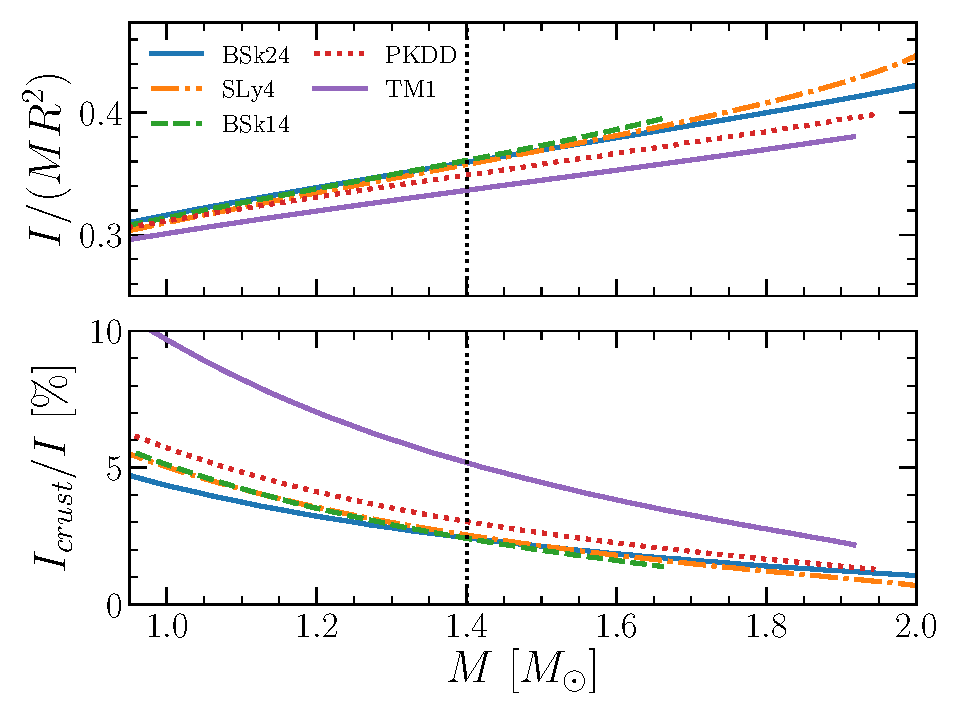
\includegraphics[width=0.9\linewidth]{figures/moi_popular.pdf}
\end{center}
\caption[Moment of inertia and fraction of crust moment of inertia
versus neutron star mass for several popular equations of state]{Moment of
  inertia $I$ (upper panel) and fraction of crust moment of inertia
  $I_{crust}/I$ (lower panel) as a function of the NS mass $M$ for several 
  popular EoS calculated within the metamodeling technique. In the upper panel, 
  the black dotted line marks the NS canonical mass, that is $1.4M_\odot$. In
the lower panel, the minimum values needed to justify Vela glitches with
(Delsate \textit{et al.}~\cite{Delsate2016} and Andersson \textit{et
al.}~\cite{Andersson2012}) and without (Link \textit{et al.}~\cite{Link1999}) 
crustal entrainment are represented.}\label{fig:moi_popular}
\end{figure}

The total moment of inertia is plotted as a function of the NS mass in the
upper panel of Fig.~\ref{fig:moi_popular} for EoS based on Skyrme-type
functionals BSk24, SLy4, and BSk14, and relativistic models PKDD and TM1.
For $M=1.4M_\odot$, it is found that $I$ ranges from $\approx 1.2\times 
10^{45}$ g cm$^2$ for the soft BSk14 EoS to $\approx 2\times 10^{45}$ g cm$^2$ 
for the very stiff TM1 EoS. This shows the strong dependence on the EoS, 
{that appears to be even larger for high-mass NS.}

The lower panel of Fig.~\ref{fig:moi_popular} shows the variation with NS mass
of $I_{crust}/I$ for the same EoS. It is seen that the more massive an 
NS is, the less moment of inertia it stores in its crust, which follows
the trends observed in Fig.~\ref{fig:crustmassthick}. This is expected from 
the sensitivity of crustal properties to the CC transition pressure. Given the 
selected EoS, the value of $I_{crust}/I$ at $M=1.4M_\odot$ 
ranges from $\approx 2\%$ for BSk14 to $\approx 5\%$ for TM1, showing once 
again the important dependence on the EoS. 
{The studies on crust properties requires a unified modeling, such as
the one introduced in Chapter 1. Nonetheless, there have been propositions to
obtain crust properties from the mere knownlege of the EoS of homogeneous 
matter and the density and pressure at the CC transition 
point~\cite{Zdunik2017}, though we have tested those methods and found that 
they are imprecise for $M \lesssim 1.2M_\odot.$}

\subsubsection{Connection to pulsar glitches}\label{subsubsec:glitch}

%The so-called pulsar glitches are sudden jumps in the rotational frequency of 
%a compact star. They are thought to originate from an abrupt transfer of 
%angular momentum from the superfluid components of the NS, acting as an angular 
%momentum reservoir, to the solid crust of the star, and all the normal fluid
%components which are strongly coupled to the crust by mutual dissipation, due 
%to the unpinning of the superfluid vortices from the crystal 
%lattice~\cite{Anderson1975}. 
%%
%A rotating superfluid, such as the superfluid neutrons in the inner crust of 
%the NS, produces individual quantized vortices, with a density proportional to 
%the rotational rate. Those vortices migrate towards the surface of the star due 
%to the centrifugal force, where they get pinned to the ions of the lattice that 
%constitutes the star solid crust. Since the star experiences a spin-down due to 
%the emission of elecromagnetic radiation, a differential lag develops between 
%the faster superfluid vortices and the slower crust, leading to crustal stress. 
%%
%When the differential lag between the slower solid crust and faster superfluid 
%vortices reach some threshold and can no longer be sustained, the vortices
%suddenly unpin from the lattice sites, leading to an angular momentum transfer
%to the crust, and the rest of the star which is entangled with the crust by
%mutual friction, so as to recover a close equilibrium between the normal and
%superfluid components. Since the electromagnetic slowing down is a continuous
%process, this is not a final equilibrium situation, and eventually stresses 
%start to build up again, ultimately leading to another glitch event.

%At the time of writing, 555 glitches have been observed in 190 pulsars through 
%high-precision pulsar timing~\cite{Espinoza2011,Glitches}. 

As discussed in the introduction, sudden spin-ups of radio pulsars, called 
glitches, are thought to be produced by angular momentum transfer from the
superfluid component of the stellar interior to the solid crust.

For a given glitcher, three quantities are usually measured: its spin frequency 
$\Omega$, its average spin-down rate $\dot{\Omega}$, and its glitch activity 
parameter $\mathcal{A}$, defined as
%
\begin{equation}
  \mathcal{A} = \frac{1}{t}\sum_{i=1}^{N} \frac{\Delta \Omega_i}{\Omega},
\end{equation}
%
where $\sum_i \Delta\Omega_i/\Omega$ represents the cumulative spin-up rate
over the $N$ glitches occurring during a time $t$.

It was demonstrated in~\cite{Link1999} that the ratio of the moment of inertia
associated to the neutron superfluid which drives the glitches $I_{sf}$ to the 
moment of inertia of the solid crust -- plus any portion of the star strongly 
coupled to it -- $I_c$ must satisfy 
%
\begin{equation}
  \frac{I_{sf}}{I_c} \geq \frac{\Omega}{|\dot{\Omega}|}\mathcal{A} 
  \equiv \mathcal{G},
\end{equation}
%
where we have introduced the coupling parameter $\mathcal{G}$. In view of
relating the observational constraint $\mathcal{G}$ to the fractional moment of
inertia $I_{crust}/I$ to ultimately set a constraint on the stellar EoS, we 
assume that the angular momentum reservoir is confined to the neutron 
superfluid coexisting with the crystal lattice of the inner crust. 
%
{This is justified by the fact that the pairing gap in PNM vanishes at
suprasaturation densities~\cite{Cao2006}.}
%
In that case, we have $I_c = I - I_{res} \simeq I$ and 
$I_{crust} \simeq I_{sf}$, yielding~\cite{Link1999}
%
\begin{equation}
  \frac{I_{sf}}{I_c} \simeq \frac{I_{crust}}{I} 
  \geq \mathcal{G}\label{eq:noent}.
\end{equation}
%

In reality, the neutron superfluid is strongly coupled to the solid crust due
to nondissipative entrainment effects~\cite{Chamel2013}, limiting the amount of
angular momentum that can be transferred during a glitch event. The importance
of the entrainment coupling is related to the neutron effective mass $m_n^*$ in
the inner crust, which is proportional to the ratio of unbound neutrons to 
those that are not entrained, $m_n^* \equiv m_n n_g/n_g^c$. Taking into 
account the entrainment effects, the previous constraint, Eq.~(\ref{eq:noent}), 
then becomes~\cite{Carter2005,Andersson2012}
%
\begin{equation}
  \frac{I_{crust}}{I} \geq \mathcal{G}\frac{\langle m_n^*
  \rangle}{m_n},\label{eq:ifrac_g}
\end{equation}
%
with $\langle m_n^* \rangle$ the average neutron effective
mass\footnote{{It is important to stress that this effective mass differs 
    from the definition Eq.~(\ref{eq:effm}), which corresponds to the $k$-mass 
    $m_{n,k}$ arising from the spatial nonlocality of the mean field. For
    transport properties, which correspond to a dynamical phenomemon, the full
    nonlocality of the interaction in space and time must be considered,
    leading to the definition of the $\omega$-mass. In this context,  the 
    neutron effective mass reads $m_n^* = m_{n,k} m_{n,\omega}/m_n$, where 
    $m_{n,\omega}$ is the $\omega$-mass.}}.
It should be stressed that systematic calculations of $m_n^*$ throughout 
the NS crust are very costly from the computational point of view. To get an 
order of magnitude of the effect, 
following~\cite{Andersson2012,Piekarewicz2014}, we adopt the 
value $\langle m_n^* \rangle /m_n = 4.3$, which is inferred from the 
results of~\cite{Chamel2012} obtained with the BSk14 functional. 
Naturally, one recover the expression without 
crustal entrainment in the case of $\langle m_n^* \rangle = m_n$. We should 
stress that the importance of the effect of crustal entrainment, that is the 
value of the average neutron effective mass throughout the solid crust, is 
currently under debate~\cite{Martin2016,Watanabe2017}.

The Vela pulsar (PSR B0833-45) is one of the most active glitchers known, with
glitches occurring four times per decade on average. Since the beginning of its 
monitoring, almost than 50 years ago, it has exhibited 20 glitches in
total~\cite{Glitches}, allowing for a precise estimation of the corresponding 
coupling parameter, $\mathcal{G}_{\text{Vela}} = (1.62 \pm 0.03) \times
10^{-2}$~\cite{Ho2015}. This can be translated into a constraint for 
the fraction of crust moment of inertia,
%
\begin{equation}
  \left(\frac{I_{crust}}{I}\right)_{\text{Vela}} \geq (1.62 \pm 0.03) \times 10^{-2}
  \frac{\langle m_n^* \rangle}{m_n} \approx 0.07.
\end{equation}
%
In other words, in the standard picture where the angular momentum reservoir is 
exclusively confined to the neutron superfluid permeating the inner crust, the 
crust must store more than $7\%$ (with entrainment effects included) of the 
total moment of inertia in order to justify the large glitches occurring in the 
Vela pulsar.

The Vela constraints on $I_{crust}/I$ are displayed in the lower panel of 
Fig.~\ref{fig:moi_popular}. Neglecting entrainment effects~\cite{Link1999}, it
is seen that the constraint is easily satisfied. For BSk14 EoS, which is the
softest EoS here, it leads to $\approx 1.6M_\odot$ for the maximum mass of 
Vela. Now including crustal entrainment with $\langle m_n^*\rangle/m_n =
4.3$~\cite{Andersson2012}, it is not clear, due to dependence on the EoS, 
whether the superfluid neutron in the crust can carry enough angular momentum 
to explain Vela glitches. For the three nonrelativistic Skyrme-based EoS that 
we consider, we see that the constraint is unlikely to be satisfied, because it
would require Vela mass to be very low, $M_{\text{Vela}} \lesssim 0.9M_\odot$.
While theoretically plausible~\cite{Haensel2007}, such low-mass NS have never 
been observed to this day. On the other hand, it is observed that very stiff 
EoS such as TM1 can be consistent with the constraint~\cite{Piekarewicz2014}.
Finally, given the constraint on the fractional moment of inertia calculated 
with the present largest estimation of crustal entrainment~\cite{Delsate2016}
(black thick line), we find that the inferred mass of Vela is at most 
$\approx 0.85M_\odot$ for the stiff TM1 EoS and $\approx 0.65M_\odot$ for the 
soft EoS based on Skyrme functionals. Clearly the question 
``\textit{Is the crust enough?}'' deserves further investigations. In that 
sense, it will be addressed in~\ref{subsec:gli_stats} in the context of a 
complete statistical analysis~\cite{Carreau2019moi}.

\subsection{Tidal deformability}\label{subsec:tidal} % 2

Theoretically, the tidal deformability parameter is the 
observable which makes the link between the EoS and the gravitational signal
associated to the coalescence of two NS.
In that sense, GW observations can ultimately provide new constraints on the 
EoS. 
In particular, the first detection of GW from the coalescence of two NS, 
the GW170817 event, has yielded important constraints for the tidal 
deformability of NS~\cite{GW1}.

Let us consider a static, spherically symmetric NS, placed in a static external
quadrupolar tidal field $\mathcal{E}_{tid}$. The induced quadrupole moment of
this star is given by 
%
\begin{equation}
  Q_{tid} = -\lambda \mathcal{E}_{tid},
\end{equation}
%
where $\lambda$ is the tidal deformability, which is related to the so-called 
tidal Love number $k_2$ by
%
\begin{equation}
  \lambda = \frac{2}{3}k_2\left(\frac{Rc^2}{G}\right)^5.
\end{equation}
%
Let us also define the dimensionless tidal deformability,
%
\begin{equation}
  \Lambda = \frac{\lambda}{M^5} = \frac{2}{3}k_2\beta^{-5},
\end{equation}
%
where we have introduced the compactness of the star $\beta = GM/(Rc^2)$.
Similarly to the moment of inertia in the slow rotation approximation, $k_2$ 
can be obtained from the solution of the following first-order differential 
equation~\cite{Hinderer2010},
%
\begin{eqnarray}
  \frac{dy}{dr} &=& -\frac{y^2}{r} - \frac{y-6}{r-2Gm/c^2} \notag\\
                &&- \frac{4\pi G}{c^2}r^2\frac{(5-y)\rho_B + (9+y)P/c^2 
                + (P+\rho_Bc^2)/c_s^2}{r-2Gm/c^2} \notag\\
                &&+ \frac{1}{r}\left[\frac{2G}{c^2}\frac{(m+4\pi p r^3/c^2)}{r 
                - 2Gm/c^2}\right]^2\label{eq:dy},
\end{eqnarray}
%
where we have introduced the speed of sound $c_s = \sqrt{\partial P/\partial 
\rho_B}$, and that must satisfy the boundary condition $y(r=0)=2$. This
equation together with the hydrostatic equilibrium equations, 
Eqs.~(\ref{eq:tov}) and~(\ref{eq:massbal}), are solved simultaneously. The 
tidal Love number reads
%
\begin{equation}
  k_2 = \frac{8}{5}\beta^5(1-2\beta)^2[2-y(R) + 2\beta(y(R) - 1)]/a,
\end{equation}
%
with
%
\begin{eqnarray}
  a &=& 6\beta[2-y(R)+\beta(5y(R)-8)] \notag\\
    &&+ 4\beta^3[13-11y(R)+\beta(3y(R)-2)+2\beta^2(1+y(R))] \notag\\
    &&+ 3(1-2\beta)^2[2-y(R)+2\beta(y(R)-1)]\ln(1-2\beta).
\end{eqnarray}
%

\begin{figure}[!t]
  \begin{center}
    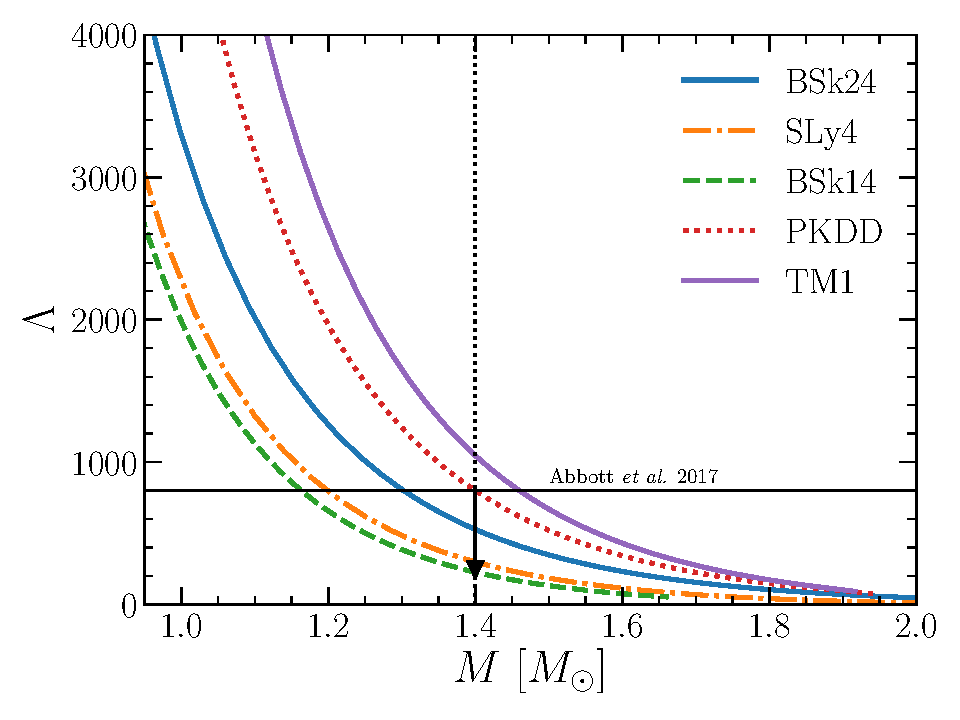
\includegraphics[width=0.9\linewidth]{figures/tidal_popular.pdf}
  \end{center}
  \caption[Tidal Love number and dimensionless tidal deformability versus 
  neutron star mass for several popular equations of state]{Tidal Love number 
    $k_2$ (upper panel) and 
    dimensionless tidal deformability $\Lambda$ (lower panel) as a function of 
    the NS mass $M$ for several popular EoS calculated within the metamodeling 
  technique. The black dotted line marks the NS canonical mass, that is
$1.4M_\odot$. In the inset of the lower panel, the value 
$\Lambda_{1.4} = 190_{-120}^{+390}$ (at $90\%$ level) inferred from GW170817 
event is represented~\cite{GW1}.}\label{fig:tidal_popular}
\end{figure}

Fig.~\ref{fig:tidal_popular} shows the variation with NS mass of $k_2$ for the 
several popular EoS that we consider in this chapter. The tidal Love number
measures how easily the bulk of the matter in an NS is deformed. In the case
of the mass being concentrated at the center of the star, the tidal deformation 
is small, and so is $k_2$. In agreement with~\cite{Hinderer2010}, we find that 
$k_2$ lies in the range $\approx 0.05-0.15$. The relative difference between
the present EoS is of the order of $\approx 35\%$ for $M=1.4M_\odot$, showing
once again the notable dependence on the EoS. {In particular, it has been
shown very recently that $k_2$ is sensitive to $L_{sym}$ but not to
$E_{sym}$~\cite{Perot2019,Perot2020}.} 
Let us also point out that the tidal Love number is very sensitive to the 
description of the crustal component of the EoS~\cite{Piekarewicz2019}. 

The dimensionless tidal deformability is plotted as a function of $M$ in the 
lower panel of Fig.~\ref{fig:tidal_popular}. In the mass range considered, it 
is seen that the more massive the NS is, the less it gets deformed when 
orbiting another massive compact object. In the inset, we show the value of
the dimensionless tidal deformability for a $1.4M_\odot$ NS inferred from the 
GW170817 event, $\Lambda_{1.4} = 190_{-120}^{+390}$ at the $90\%$ level. We can
observe that the EoS which predict the largest tidal effects, PKDD and TM1, are 
unlikely. One can notice the tension between the evidence of a rather soft 
EoS, typically satisfied by nonrelativistic Skyrme-type functionals, which 
predict small tidal deformations, and the need of a rather stiff EoS, typically 
obtained in the framework of relativistic models, to explain the glitch 
phenomenon as well as the most massive NS.

\section{Bayesian determination of the equation of state
parameters}\label{sec:bayes}

In recent years, there has been a lot of efforts invested in the development of
the chiral EFT~\cite{Drischler2016} with the aim of 
providing new constraints on the low-density EoS. As we have already discussed, 
the maximum observed mass of NS~\cite{Antoniadis2013,Cromartie2020} establishes 
a stringent constraint on the EoS. Furthermore, and for the same
reason, future observations of GW signatures associated to binary NS mergers 
with LIGO and Virgo, and radius measurements from NICER will beneficial.
Bayesian inference is a statistical method which allows to account both for the 
present day knowledge on nuclear physics and NS observables for predicting the 
stellar matter EoS.

This section deals with the Bayesian determination of the EoS
parameters. The general formalism of Bayesian inference is recalled and its
application for constraining the EoS is explained in~\ref{subsec:bayes}.
In~\ref{subsec:prior}, we give the prior distribution of EoS parameters
and a sensitivity analysis of the CC transition point is carried out 
afterwards. The likelihood function, based on constraints on nuclear physics
observables, constraints on NS observables, and physical requirements, is 
constructed in~\ref{subsec:likeli}. Finally, we present the posterior 
distribution of empirical parameters in~\ref{subsec:posterior}. A particular 
attention is paid to the correlations among parameters.

\subsection{Principle of Bayesian inference}\label{subsec:bayes}

The core of Bayesian inference is based on well-known Bayes' theorem, 
which provides an expression for the conditional probability (or posterior
probability) of a set of values for an ensemble of random variables $A$ given a
second set $B$,
%
\begin{equation}
  P(A|B) = \frac{P(B|A)P(A)}{P(B)}.
\end{equation}
%
In this equation, $P(B|A)$ is the conditional probability of $B$ given $A$, 
$P(A)$ is the prior probability of $A$, and $P(B)$ that of $B$. 
The key point of the method is to realize that random variables are not limited
to observational data, but they can comprise unknown parameters entering a
theoretical modeling (the EoS parameters in our case). 
In this model form of Bayes' theorem, one replaces $B$ by data, $A$ with 
a parameter set $\bm{X}$, and $P$ with probability density functions (PDF) 
$p$, resulting in~\cite{Bayes}
%
\begin{equation}
  p(\bm{X}|\text{data}) = \frac{p(\text{data}|\bm{X})
  p(\bm{X})}{p(\text{data})}.\label{eq:bayes1}
\end{equation}
%
The denominator acts as a normalization constant which makes 
sure that the posterior distribution $p(\bm{X}|\text{data})$ is a 
true probability distribution, by ensuring that the sum of the distribution is 
equal to 1. It is given by
%
\begin{equation}
  p(\text{data}) = \int p(\text{data}|\bm{X})p(\bm{X})
  d\bm{X}.
\end{equation}
%
The model-based formulation of Bayes' theorem, Eq.~(\ref{eq:bayes1}), is 
therefore often written as
%
\begin{equation}
  p(\bm{X}|\text{data}) \propto p(\text{data}|\bm{X})
  p(\bm{X}).
\end{equation}
%
The marginal one- and two-parameter posterior distributions can be extracted
from the posterior distribution. Then are defined respectively as
%
\begin{eqnarray}
  p(X_j|\text{data}) &=& \left\{\prod_{i \neq j} \int
  dX_i\right\}p(\bm{X}|\text{data}),\label{eq:marg1}\\
  p(X_j,X_k|\text{data}) &=& \left\{\prod_{i \neq j,k} 
    \int dX_i\right\}p(\bm{X}|\text{data}).
\end{eqnarray}
%

Let us describe the different components of Bayesian inference. The 
prior distribution $p(\bm{X})$ represents our knowledge or bias on the 
model parameters, prior to the measurement noted ``data''. It can thus be more 
or less informative.
$p(\text{data}|\bm{X})$ is the likelihood of observing the data given the model
parameters $\bm{X}$. It is determined from the data comparison between the 
model and the measurement via an error estimator. In that sense, the link 
between the data and the model parameters is encoded in the likelihood
distribution. 
Multiplying the prior by the likelihood function, one obtains the unnormalized 
joint posterior PDF, which corresponds to the conditional distribution of 
model parameters $\bm{X}$ given the data. Let us notice that the prior 
distribution obviously affects the posterior distribution, implying that it has
to be handled with care, and the choice of the prior is the most delicate part
of the method. 

Bayesian inference is an appealing statistical method in the sense that it 
allows to calculate the joint posterior distribution of model parameters using 
prior beliefs updated with the likelihood. In the context of NS physics, and 
from the nuclear physicist point of view, it allows for instance to update our 
knowledge on the nuclear EoS by taking into consideration the data arising from 
various astrophysical observations, that are for example the NS mass inferred
from Shapiro delay or the tidal deformability from GW measurements.
Conversely, one can account for nuclear physics constraints in the prediction 
of macroscopic observables related to NS. 
In our case, we first generate a large number of EoS, each of them being 
defined by a set of parameters $\bm{X}$, to numerically sample the prior 
parameter distribution. Then, we filter those EoS through constraints, which 
arise from physical requirements, astrophysical observations, and ab initio
calculations of SNM and PNM. This 
gives us the joint posterior distribution of model parameters, from which we 
can finally calculate the posterior EoS and make general predictions for NS 
observables. Those predictions are presented in Section~\ref{sec:general}.

Let us describe the parameter set $\bm{X}$. Our calculation
of the stellar EoS is based on the metamodeling of nuclear matter
energy~\cite{Margueron2018a} introduced in~\ref{subsubsec:hnm}. The empirical
parameters $E_{sat}$, $n_{sat}$, $K_{sat}$, $Q_{sat}$, $Z_{sat}$, $E_{sym}$,
$L_{sym}$, $K_{sym}$, $Q_{sym}$, and $Z_{sym}$ -- which we recall are given by 
the successive derivatives of the NM energy at saturation density in isoscalar 
and isovector sectors -- therefore 
enter into the parameter set. The parameter $b$ is also added in order 
to explore different functional behaviors close to the $n\rightarrow 0$ limit. 
{This is motivated by the fact that the behavior of Skyrme-type 
functionals is not correct at extreme low densities~\cite{Grasso2017}.}
The parameter $b$, together with the isoscalar effective mass $m_{sat}^*/m$ and 
isospin splitting $\Delta m_{sat}^*/m$, completes the parameter space, 
associated to the description of bulk matter.
In the solid crust, the metamodeling technique is supplemented by a surface 
plus curvature term in order to describe the surface properties of finite 
nuclei. Thus, one could consider adding the surface and curvature parameters, 
respectively $\sigma_0$, $b_s$, $p$, and $\sigma_{0c}$, $\beta$, as extra
parameters to $\bm{X}$. However, we have
seen in Fig.~\ref{fig:surf_fit} that the $\chi^2$ function, which evaluates the 
goodness of the fit of those parameters to experimental nuclear masses given 
BSk24 empirical parameters and $p=3$, is strongly peaked on a given set
$\bm{S}=\bm{S_{opt}}$. This feature is generic and not limited to BSk24, and we 
therefore choose to not include 
the surface and curvature parameters in $\bm{X}$ but to take the set 
$\bm{S_{opt}}$ that minimizes $\chi^2$, as explained in~\ref{subsubsec:cld}.
It is important to stress that, even if we keep only the optimized values for
the surface and curvature parameters for each parameter set, a large parameter
space is explored for the surface energy because of the large variation of the 
bulk properties and the physical correlation between surface and bulk due to 
the fit to experimental data.
We consider two choices for the value of the parameter $p$, which determines 
the behavior of the surface tension for extreme isospin values. Either it is 
fixed to the educated value $p=3$, or $p=\{2.5,3,3.5\}$ is selected for each
set of empirical parameters. The latter option is considered for the
determination of observables that are sensitive to the CC transition point, 
which we have seen is strongly correlated to the isovector properties of the 
surface tension.

\subsection{Prior distribution of equation of state parameters}\label{subsec:prior}

We now discuss the prior distribution of empirical parameters. We first give 
insights concerning the selected intervals for the flat prior. A sensitivity 
analysis of the CC transition point is performed afterwards.

\subsubsection{Flat prior compatible with empirical constraints}\label{subsubsec:prior}

\begin{table}[!t]
  \begin{center}
    \begin{tabular}{ccccc} 
      \toprule
      \toprule
      Parameter & Unit & $N$ & Min & Max \\
      \midrule
      $E_{sat}$ & MeV & 0         & -17   & -15  \\
      $n_{sat}$ & fm$^{-3}$ & 1   & 0.15  & 0.17 \\ 
      $K_{sat}$ & MeV & 2         & 190   & 270  \\ 
      $Q_{sat}$ & MeV & 3         & -1000 & 1000 \\ 
      $Z_{sat}$ & MeV & 4         & -3000 & 3000 \\ 
      $E_{sym}$ & MeV & 0         & 26    & 38   \\
      $L_{sym}$ & MeV & 1         & 10    & 80   \\
      $K_{sym}$ & MeV & 2         & -400  & 200  \\
      $Q_{sym}$ & MeV & 3         & -2000 & 2000 \\
      $Z_{sym}$ & MeV & 4         & -5000 & 5000 \\
      $m_{sat}^*/m$ & &           & 0.6   & 0.8  \\
      $\Delta m_{sat}^*/m$ & &    & 0.0   & 0.2  \\
      $b$ & &                     & 1     & 10   \\
      \bottomrule
      \bottomrule
    \end{tabular}
  \end{center}
  \caption[Minimum value and maximum value of each of the empirical parameters
  for the prior distribution]{Minimum value and maximum value of each of the
    parameters of parameter set $\bm{X}$. The associated unit and derivative 
  order $N$ are also reported.}\label{table:prior}
\end{table}

The prior distribution of $\bm{X}$ is given by an uncorrelated ansatz and an
uniform distribution of each parameter within the interval specified in
Table~\ref{table:prior},
%
\begin{equation}
  p(\bm{X}) = \prod_{i=1}^{2(N+1)+3} \mathcal{U}(X_i^{min}, X_i^{max};X_i),
\end{equation}
%
where the parameter $X_i$ is uniformly distributed from $X_i^{min}$ to 
$X_i^{max}$. The use of a flat prior means that all possible values of 
$\bm{X}$ inside the intervals are equally likely a priori.

The range of variation for the model parameters reflect the degree of 
uncertainty on the EoS parameters, as measured by their variation in the 
functionals which reproduce successfully low energy nuclear physics
data~\cite{Margueron2018a}. We can distinguish three groups of empirical  
parameters, depending on how well they are experimentally constrained. The 
first group consists of the low-order isoscalar parameters $E_{sat}$, 
$n_{sat}$, $K_{sat}$, the symmetry energy at saturation density $E_{sym}$, as 
well as the effective mass $m_{sat}^*$ and isospin splitting 
$\Delta m_{sat}^*/m$. These parameters are rather well determined by nuclear 
experiments, with associated relative uncertainties lower than $15\%$. The 
second group consists of the parameters that are still poorly determined by 
nuclear experiments. The uncertainties on the isoscalar skewness $Q_{sat}$, the 
slope of the symmetry energy $L_{sym}$, and the isovector incompressibility 
$K_{sym}$ are very large, yet one can expect a better accuracy to be 
reached in the near future. In particular, the determination of $L_{sym}$ is 
an highly topical issue nowadays~\cite{Li2014}. Finally, the last group 
concerns the parameters which are inaccessible to nuclear experiments to the 
present day, that is the isovector skewness $Q_{sym}$ as well as the parameters 
of order $N=4$, $Z_{sat}$ and $Z_{sym}$. As a consequence, we explore very 
large ranges for these parameters. 
The choice of the interval for the low-density parameter, $b = [1,10]$, is 
discussed thoroughly in~\cite{Antic2019}. {In this paper, we have 
  investigated the influence of the uncertainties of the EoS parameters on the
CC transtion point, calculated using the dynamical method with the ETF
approach for the surface contribution. We have considered a Bayesian framework
with the same prior distribution of empirical parameters and likelihood 
function as in this thesis, and we have found that $K_{sym}$ and $Q_{sym}$ have 
the most significant correlations with the transition density and pressure.}

\subsubsection{Sensitivity analysis of the crust-core transition
point\footnote{Partial results of the presented work have been published in 
Eur. Phys. J. A (2019) \textbf{55}: 188. With kind permission of The European
Physical Journal (EPJ).}}\label{subsubsec:sensana}

Let us recall that one of the advantages of the metamodeling approach is that 
all the EoS model parameters, such as the empirical parameters, are a priori
uncorrelated. 
It is therefore possible to vary each one of them independently of the others, 
which is not feasible using specific functional behaviors such as Skyrme, 
Gogny, or the different versions of RMF, as discussed in detail
in~\cite{Margueron2018a,Margueron2019}. 
Indeed, common functionals describing infinite NM have a smaller number of 
parameters compared to the metamodel, which creates a priori correlations that 
are not fully controlled. If we take the example of Skyrme forces, the density 
dependence of SNM is controlled by only three parameters, which are fixed 
to reproduce the coordinates of the saturation point: $n_{sat}$, $E_{sat}$, and 
$K_{sat}$. Thus, the isoscalar skewness $Q_{sat}$ is correlated with the 
three other parameters, and it turns out that this correlation is not the same, 
for instance, in Skyrme, Gogny, or in RMF functionals~\cite{Margueron2019}. A 
similar argument applies to the symmetry energy: when the density dependence of 
the symmetry energy is governed by a single parameter as for example often 
assumed in heavy ion 
transport models, an isosoft behavior at suprasaturation density is necessarily 
associated to an isostiff behavior at subsaturation density, while more 
complicated behaviors are possible~\cite{Margueron2019}. The independent 
variation of the different empirical parameters allows a simple determination 
of the most influential parameters impacting a given observable under study. 

\begin{figure}[!t]
\begin{center}
  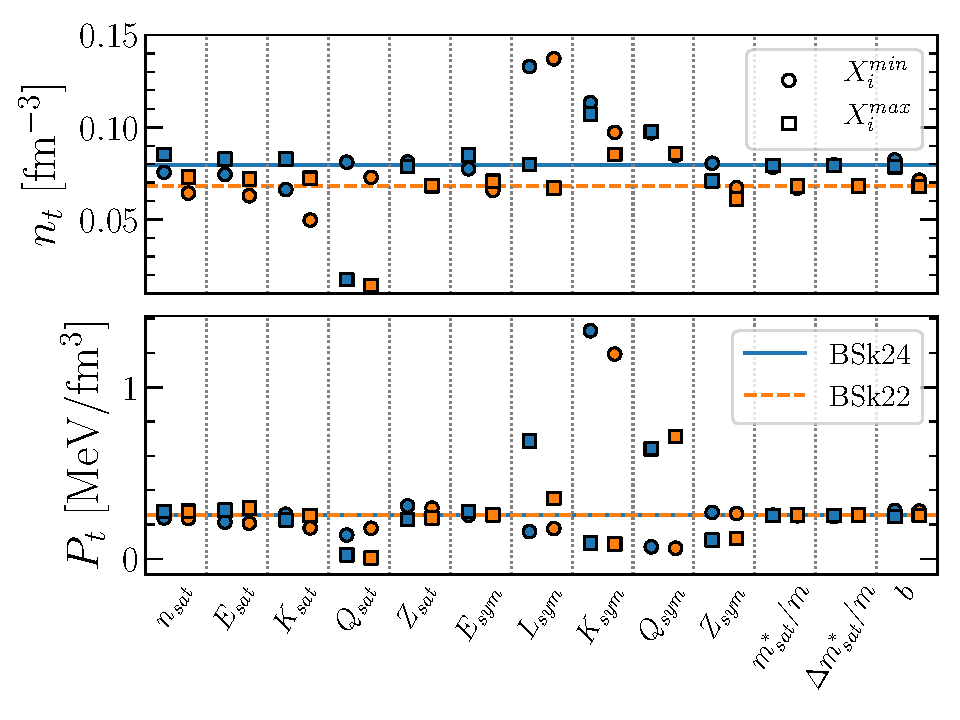
\includegraphics[width=0.9\linewidth]{figures/sensana.pdf}
\end{center}
\caption[Sensitivity analysis of the crust-core transition point for
BSk24 and BSk22]{Sensitivity analysis of the transition density $n_t$ (upper 
panel) and transition pressure $P_t$ (lower panel) with respect to EoS 
parameters. $p=3$ is fixed and two different reference point are chosen:
BSk24 parameters (solid blue lines) and BSk22 parameters (orange 
dashed lines). For each parameter, the symbols on left (blue) correspond to 
BSk24 and those on right (orange) to BSk22. Circles and squares are
respectively associated to the minimum value $X_i^{min}$ and maximum value
$X_i^{max}$ of the parameter, which are listed in 
Table~\ref{table:prior}.}\label{fig:sensana}
\end{figure}
 
Such a sensitivity analysis is presented in Fig.~\ref{fig:sensana} for the 
CC transition density $n_t$ and transition pressure $P_t$. The reference 
metamodel used in the sensitivity analysis can have an influence. For this 
reason, the sensitivity analysis varying one by one the EoS parameters is 
performed around two different reference parameter sets $\bm{X_{ref}}$, namely 
the parameter set corresponding to the BSk24 functional (solid blue lines), and 
the one corresponding to the BSk22 functional 
(dashed orange lines)\footnote{Other choices can be found 
  in~\cite{Carreau2019cc}, leading to same qualitative results.}.
For both of sets of parameter, we fix $p=3$ as well as $b=10\ln(2)$.

The range of variation for each of the EoS parameters corresponds to the 
intervals for the prior distribution $p(\bm{X})$ specified in 
Table~\ref{table:prior}. Let us however notice that some sets produce nonviable 
EoS, for which a solution for the CC transition point cannot be found. This
occurs in particular when varying the value of the isovector incompressiblity 
parameter $K_{sym}$ with BSk24 as reference parameter set. Indeed, we find 
an extremely soft behavior for the symmetry energy for the minimum value 
$K_{sym}^{min}=-400$ MeV. In that very situation, we increase the minimum value 
of the parameter to $K_{sym}^{min} \approx -300$ MeV so as to find a solution 
for $n_t$ and $P_t$.

The symbols in Fig.~\ref{fig:sensana} give the transition density and 
pressure domain obtained when the EoS parameters are one by one varied around 
the reference model, within the interval of Table~\ref{table:prior}. More
specifically, circles and squares are respectively associated to the minimum
value and maximum value of each parameter.
Since the uncertainty on the different parameters is not the same, the 
relative distance between circles and squares is a qualitative measurement of 
the propagation of the uncertainty on the transition point brought by each 
parameter. We can see that the sensitivity of each parameter depends on the 
value of the other parameters, that is on the chosen reference set 
$\bm{X_{ref}}$. Still, universal trends clearly emerge. We can see that the CC 
phase transition, at variance with the 
standard liquid-gas of SNM, is almost insensitive to isoscalar parameters. 
In particular, the influence of the isoscalar parameters in the 
transition pressure is almost negligible, and only the third derivative term 
$Q_{sat}$ is influential on $n_t$. This underlines the importance of 
the energetics of the neutron gas on the transition point. Concerning the 
isovector sector, we can see that $L_{sym}$ is the most important 
parameter as far as the transition density is concerned. This result is in 
agreement with previous findings by many authors~\cite{Ducoin2011} and was
already anticipated in~\ref{subsec:ccfromc}.
The symmetry energy at saturation $E_{sym}$ and the effective mass splitting
$\Delta m_{sat}^*/m$ do not play any role on the transition. 
{This can be understood from the fact that the symmetry energy at
saturation is already relatively well constrained, and that the effective mass 
enters the kinetic energy, thus at equilibrium variations of 
$\Delta m_{sat}^*/m$ are compensated by variations of the density derivatives.} 
The transition density and pressure show also a great 
sensitivity to the isovector incompressibility parameter $K_{sym}$. 
This can explain why the transition pressure exhibits an irregular behavior 
when plotted as a function of $L_{sym}$ (see Fig.~\ref{fig:cctp_lsym}): the 
different functionals considered in the literature have very different values 
of $K_{sym}$, which blurs the correlation with $L_{sym}$. This effect is also 
amplified by the fact that, depending on the reference point, the dependence of 
$P_t$ with $L_{sym}$ is not monotonic. Finally, we can notice that the 
influence of the fully unknown high-order derivatives $Q_{sym}$ and $Z_{sym}$, 
though less important than the one of $L_{sym}$, is not negligible and 
comparable to the one of the isovector surface energy parameter $p$ that can be 
inferred from Fig.~\ref{fig:cctp_lsym}. We have checked that similar 
conclusions can be drawn if the sensitivity analysis is performed using the 
definition of the transition point from the dynamical 
spinodal~\cite{Antic2019}.

\subsection{Determination of the likelihood function}\label{subsec:likeli}

The likelihood function corresponds to the probability of observing the data
given the model parameters $\bm{X}$. In the context of our analysis, it is
defined as
%
\begin{equation}
  p(\text{data}|\bm{X}) = w_{LD}(\bm{X}) \times 
  w_{HD}(\bm{X}) \times p_{\text{AME2016}}(\bm{X}).\label{eq:likelihood}
\end{equation}
%
In this expression, $w_{LD}$ and $w_{HD}$ are strict filters that concentrate
on constraining the low-density EoS and high density EoS, respectively. Both 
filters are given by sharp $\delta$ functions that output $1$ if the constraint 
is satisfied, and $0$ otherwise. 
Constraints on nuclear physics observables, yielding the filter $w_{LD}$ and 
the probability $p_{\text{AME2016}}$ are presented in~\ref{subsubsec:ldconst}.
In~\ref{subsubsec:hdconst}, we present the
constraints corresponding to the filter $w_{HD}$, which are associated to 
general physical requirements and measurements of NS observables. 

\subsubsection{Constraints on nuclear physics
observables}\label{subsubsec:ldconst}

Let us concentrate first on the strict filter $w_{LD}$, hereafter referred to 
as low-density (LD) filter. It is introduced to verify whether the metamodel 
associated to a set of parameter $\bm{X}$ is compatible with the recent chiral
EFT calculations for SNM and PNM by Drischler 
\textit{et al.}~\cite{Drischler2016}. The authors have calculated the energy
per particle for several values of isospin at low density within the many-body
perturbation theory, based on a set of seven different Hamiltonians with chiral 
NN and three-nucleon interactions.

\begin{figure}[!t]
\begin{center}
  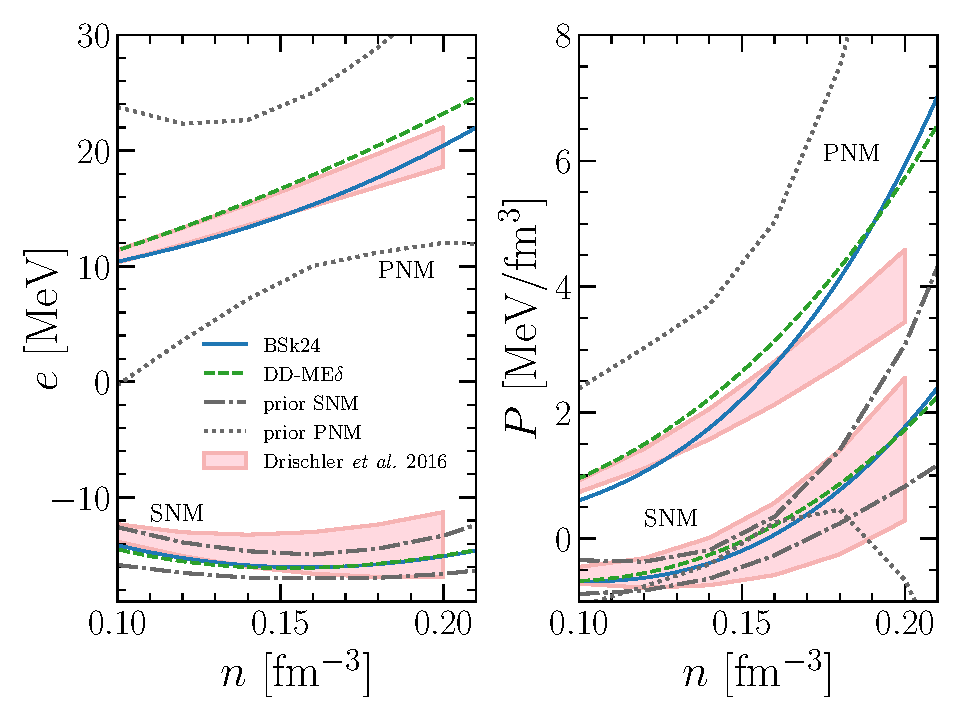
\includegraphics[width=0.9\linewidth]{figures/drischler.pdf}
\end{center}
\caption[Energy per nucleon and pressure of nuclear matter versus density from 
chiral effective field theory caclulations]{Energy per nucleon 
  (left panel) and pressure (right panel) as a function of density for both SNM 
  and PNM from chiral ETF calculations of~\cite{Drischler2016} (pink
bands). The predictions of BSk24 and DD-ME$\delta$ functionals are represented 
in solid blue lines and dashed green lines, respectively. The gray lines
give the minimum and maximum values of the prior 
distribution.}\label{fig:drischler}
\end{figure}

The resulting predicted bands for energy per nucleon as well as pressure of SNM
and PNM are shown in Fig.~\ref{fig:drischler} (pink bands), together with 
the predictions of the popular BSk24 (solid blue lines) and DD-ME$\delta$ 
(green dashed lines) functionals. 
The fact that the seven different Hamiltonians lead to different predictions
shows that the ab initio calculation is associated to a PDF exactly like an
experimental measurement. For this reason, in principle one should not apply a
strict filter but rather a likelihood one based on the PDF. The PDF being
unknown, this is however practically not feasible, and this is why we employ a
strict filter. 
The pressure band is calculated by taking the density derivative of the energy 
per nucleon for the seven Hamiltonians, thus only few density dependencies of 
the pressure are explored. 
%
In other terms, because of the uncertainty propagation taking the derivative, 
the width of the pressure band does not correspond to the same likelihood than 
the width of the energy band. Assuming that the energy band corresponds to a 
$k$-$\sigma$ surface (with $k$ unknown), we expect that if we would calculate 
the same $k$-$\sigma$ pressure surface from the energy PDF, it would be larger 
than the band of Fig.~\ref{fig:drischler}. 
%
This can explain why even realistic models such as 
BSk24 are not compatible with the theoretical band for the 
pressure of PNM above $\approx n_{sat}$. It is therefore debatable whether 
we should add the chiral EFT bands for pressure of NM in our list of
constraints defining our pass-band filters $w_{LD}$. In the following, we will 
not consider this particular constraint by default, yet we will still 
investigate how it affects the posterior distribution EoS in~\ref{sec:general}.
In the context of the pass-band filter $w_{LD}$, the chiral ETF predicted 
bands are widened by $5\%$ in order to account for other existing ab initio 
calculations in an effective manner. In addition, we will not apply the filter
in the low-density region $n < 0.10$ fm$^{-3}$ because the width of the band 
becomes extremely small, causing numerical issues.

The minimum and maximum values of the prior distribution are also
represented in Fig.~\ref{fig:drischler} (gray lines). Let us notice that one 
can infer the posterior band graphically by the comparison with the chiral 
ETF bands. Interestingly, the graphically inferred posterior band of the 
prior energy per nucleon and pressure of SNM around saturation density is 
narrower than the one corresponding to the ab initio calculation. The reason is
that low energy nuclear physics experiments provide strong empirical
constraints for SNM~\cite{Margueron2018a}, which have been embedded 
effectively in the intervals for the empirical parameters of the prior
distribution in Table~\ref{table:prior}. The same is not true for the PNM case. 
Indeed, the present day knowledge on the empirical parameters of the 
isovector sector is insufficient. For this reason, we can see that the 
corresponding ab initio bands are very thin in comparison to the prior 
distribution.

% pame2016
We now turn to the calculation of the probability $p_{\text{AME2016}}$, which 
describes the ability of the CLDM defined from a parameter set $\bm{X}$, to fit 
the measured nuclear masses of the AME2016~\cite{Huang2017}. The goodness of 
fit is evaluated by the reduced $\chi^2$, Eq.~\ref{eq:chi2}. We can define the 
associated likelihood probability as
%
\begin{equation}
  p_{\text{AME2016}}(\bm{X}) =
  \exp\left[-\frac{1}{2}\chi_\nu^2(\bm{X})\right].\label{eq:pame}
\end{equation}
%
 
\subsubsection{Physical requirements and constraints on neutron star 
observables}\label{subsubsec:hdconst}

The filter $w_{HD}$, hereafter referred to as high density (HD) filter, is
applied subsequently to the LD filter $w_{LD}$. It imposes general physical 
constraints to the global density behavior of the functional, as follows:
%
\begin{itemize}
  \item the positiveness of the symmetry energy at all densities,
  \item the stability of the EoS,
  \item the causality condition, $0 < c_s/c < 1$,
  \item the maximum observed NS mass, $M_{max}(\bm{X}) \geq M_{max}^{obs}$,
\end{itemize}
%
where $M_{max}(\bm{X})$ is the maximum mass supported by the EoS calculated for 
a parameter set $\bm{X}$, and $M_{max}^{obs}$ is the maximum observed NS mass. 
By default we choose $M_{max}^{obs} = 1.97M_\odot$, which corresponds to 
a $1\sigma$ conservative estimate, based on the observation of PSR 
J0348+0432~\cite{Antoniadis2013}. 
Let us however notice that it does not correspond to the mass of the heaviest 
NS observed to the present day~\cite{Cromartie2020}. The reason is that the
observation of PSR J0740+6620 with $M = 2.14_{-0.09}^{+0.10}M_\odot$ is very 
recent and it was not yet published at the time of this study. 
Since this measurement is affected by nonnegligible error bars, an
implementation of this extra constraint should be done using a likelihood
filter as in Eq.~(\ref{eq:pame}).

% As we have already discussed, for a given functional, the redefinition of 
% high-order parameters $Q_{sat}$, $Z_{sat}$, $Q_{sym}$, and $Z_{sym}$ is 
% necessary in order to achieve faster convergence at high density and thus 
% to recover the right value for the maximum mass. 
% The LD filter is applied in the density range $0.10$ fm$^{-3}$ $< n < 0.20$ 
% fm$^{-3}$, that is in the vicinity of the saturation density $n_{sat}$. 
% In this density range, the effect of parameters of orders $N \geq 2$ on the 
% energy per nucleon of NM is very small, and consequently we can legitimately 
% expect that $Q_{sat}$, $Z_{sat}$, $Q_{sym}$, and $Z_{sym}$ will not be strongly
% constrained by the LD filter. In that sense, for each parameter set passing 
% through the pass-band filter $w_{LD}$, we sample $10$ new parameter sets by 
% randomly drawing new values for the high-order parameters with the aim of 
% obtaining more sets passing through both LD and HD filters.
% Nevertheless, we have seen in Fig.~\ref{fig:sly4_nt} that the inclusion of
% orders $N \geq 2$ is important to precisely estimate the CC transition point.
% In that sense, $n_t$ and $P_t$ will be calculated using the high-order 
% parameters that originate from the passage through the LD filter and which are 
% kept by the HD filter.

The possibility of a negative symmetry energy at high density was sometimes 
mentioned in the literature~\cite{Li2017,Wiringa1988}. 
However, extremely soft functionals are generally incompatible with the maximum 
mass constraint, thus relaxing the condition of the positiveness of the 
symmetry energy would not alter our results.

Finally, let us notice that we do not include the constraint on the tidal
deformability inferred from the GW170817 event~\cite{GWtidal} in the $w_{HD}$ 
filter, the reason being that we are interested in confronting our results with 
the observations of LIGO and Virgo.

\subsection{Posterior distribution of equation of state 
parameters}\label{subsec:posterior}

We now turn to the description of the joint posterior distribution of equation 
of state parameters. The effect of the different filters on 
marginalized one-parameter probabilities both for isoscalar and isovector 
parameters is analyzed in~\ref{subsubsec:marg}. Correlations among empirical 
parameters are extracted from the Bayesian analysis in~\ref{subsubsec:corr}.

\subsubsection{Marginalized one-parameter posterior distributions of empirical
parameters}\label{subsubsec:marg}

The marginal one-parameter probabilities can be evaluated from the joint
posterior distribution $p(\bm{X}|\text{data})$ using Eq.~(\ref{eq:marg1}).
The generated PDF for isoscalar and isovector empirical parameters of 
orders $N\leq 3$ are shown in Fig.~\ref{fig:is_dist} and~\ref{fig:iv_dist},
respectively. The effect of the different filters on the one-parameter PDF can
be seen. We find that the likelihood probability $p_{\text{AME2016}}$,
originating from the mass fit, has a negligible impact on the distributions.
This can be understood from the fact that the prior distribution of empirical
parameters already contains information provided by nuclear experiments. Hence, 
in all cases, the probability $p_{\text{AME2016}}$ is accounted for in the
evaluation of the PDF. The isovector surface tension parameter $p$ is fixed to
be $p=3$ for this study, but the results presented in the following are 
unmodified if $p$ is allowed to vary. The reason is that $p$ is decoupled by 
construction from the homogeneous EoS parameters, and it additionally does not 
play any role in the mass fit, see Fig.~\ref{fig:surf_fit}, meaning that it is 
also independent of the other surface parameters. Five combinations of filters 
are considered:
%
\begin{itemize}
  \item the LD only without the constraint on pressure (solid blue
    lines),
  \item the LD filter only with the constraint on pressure (dashdotted blue
    lines),
  \item the HD filter only with $M_{max}^{obs} =
    1.97M_\odot$~\cite{Antoniadis2013} (solid orange lines),
  \item the HD filter only with $M_{max}^{obs} =
    2.05M_\odot$~\cite{Antoniadis2013} (dashdotted orange lines),
  \item both LD and HD filters with the constraint on pressure, for 
    $M_{max}^{obs} = 1.97M_\odot$ (solid green lines).
\end{itemize}
%

\begin{figure}[!t]
\begin{center}
  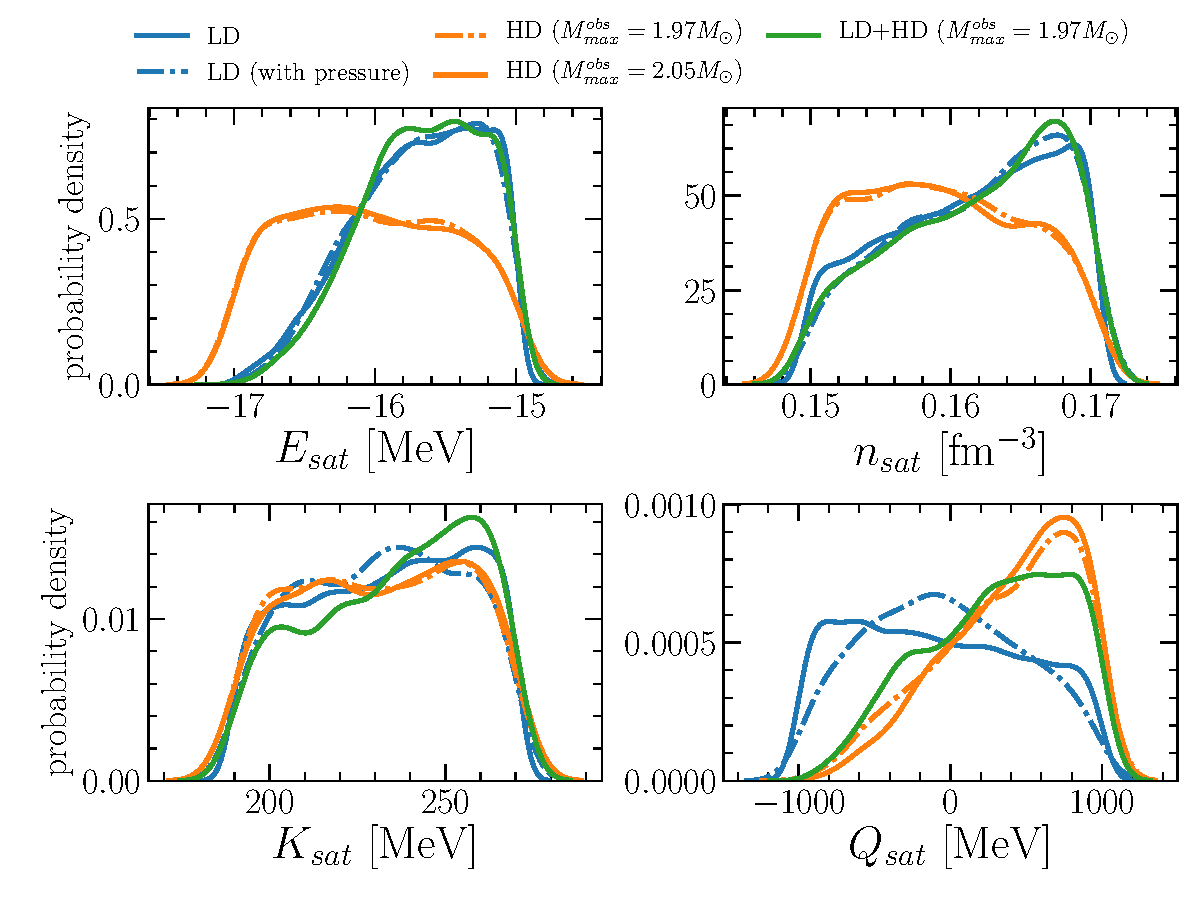
\includegraphics[width=1.0\linewidth]{figures/is_dist.pdf}
\end{center}
\caption[Marginalized posteriors for isoscalar empirical parameters assuming
different filters]{Marginalized posteriors for $E_{sat}$, $n_{sat}$, $K_{sat}$, 
and $Q_{sat}$ for the sets passing through the LD filter without (solid blue
lines) and with (dashdotted blue lines) the constraint on pressure, HD
filter with $M_{max}^{obs}=1.97M_\odot$~\cite{Antoniadis2013} (solid orange
lines) and with $M_{max}^{obs}=2.05M_\odot$~\cite{Cromartie2020}
(dashdotted orange lines), and both filters without the constraint on 
pressure, for $M_{max}^{obs}=1.97M_\odot$ (solid green lines). In all cases, 
the likelihood probability $p_{\text{AME2016}}$ is accounted for and $p=3$ is 
fixed.}\label{fig:is_dist}
\end{figure}
 
\begin{figure}[!t]
\begin{center}
  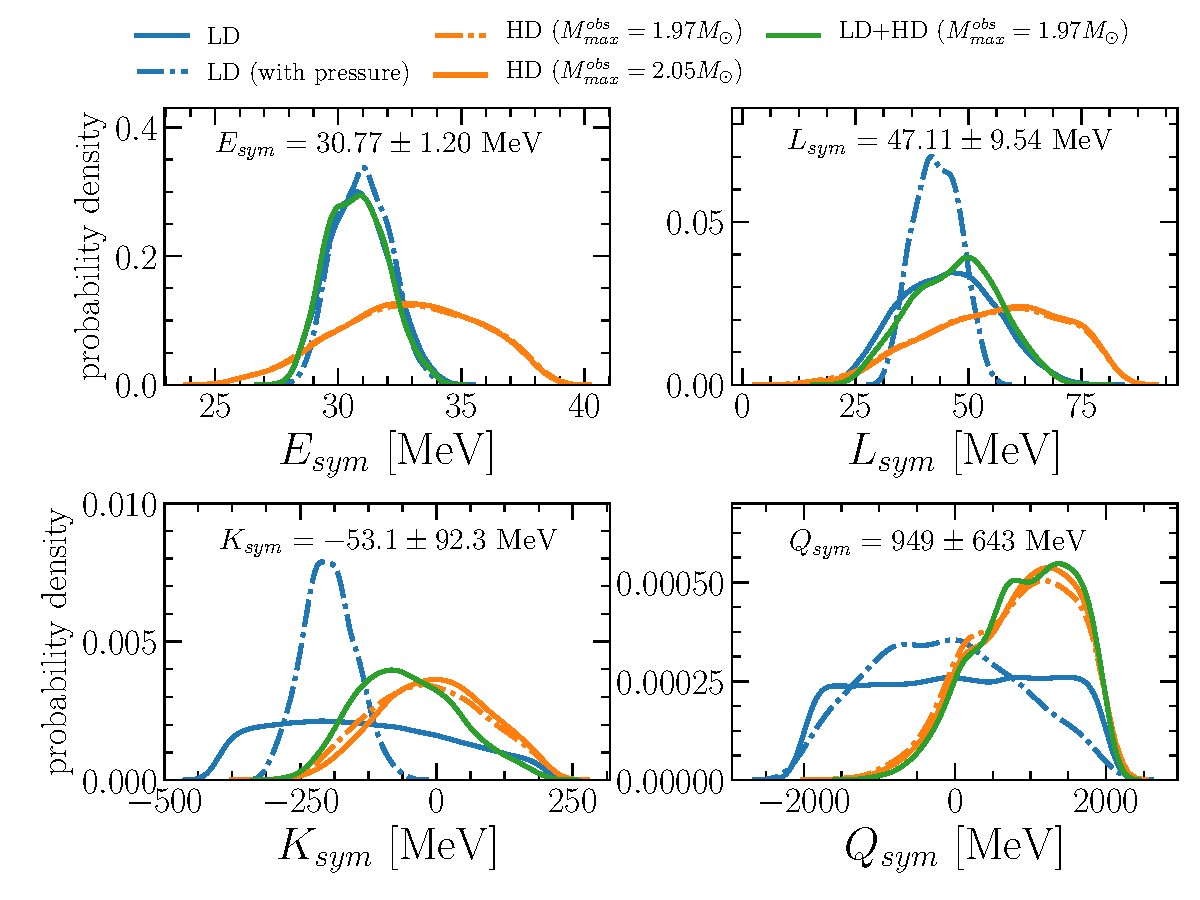
\includegraphics[width=1.0\linewidth]{figures/iv_dist.pdf}
\end{center}
\caption[Marginalized posteriors for isovector empirical parameters assuming
different filters]{Marginalized posteriors for $E_{sym}$, $L_{sym}$, $K_{sym}$, 
and $Q_{sym}$ for the sets passing through the LD filter without (solid blue
lines) and with (dashdotted blue lines) the constraint on pressure, HD
filter with $M_{max}^{obs}=1.97M_\odot$~\cite{Antoniadis2013} (solid orange
lines) and with $M_{max}^{obs}=2.05M_\odot$~\cite{Cromartie2020}
(dashdotted orange lines), and both filters without the constraint on 
pressure, for $M_{max}^{obs}=1.97M_\odot$ (solid green lines). The resulting 
mean value and uncertainty, corresponding to the latter option, are shown for 
each parameter. In all cases, the likelihood probability $p_{\text{AME2016}}$ 
is accounted for and $p=3$ is fixed.}\label{fig:iv_dist}
\end{figure}
 
By comparing the LD predictions in Fig.~\ref{fig:is_dist}, it is seen that 
adding the pressure bands, predicted by chiral EFT~\cite{Drischler2016}, as a 
constraint has a negligible effect on the posterior distributions of isoscalar
empirical parameters. Since empirical information is available in SNM and
included in our prior distribution, we observe that applying the LD filter 
does not impose strong constraints on the one-parameter PDF in the isoscalar 
sector. Still, we can notice that low values of $E_{sat}$ and $n_{sat}$ are 
disfavored by the passage through the chiral EFT predicted bands shown in 
Fig.~\ref{fig:drischler}. Conversely, it is clear from Fig.~\ref{fig:iv_dist} 
that applying LD constraints on the energy per nucleon has a enormous effect 
on the marginalized posterior distributions of the low-order isovector 
empirical parameters $E_{sym}$ and $L_{sym}$, shown in the two upper panels. 
The effect on the posterior PDF of $L_{sym}$ is even larger if we impose the 
sets to be compatible with the chiral EFT predicted bands for pressure of SNM 
and PNM. 
It also allows very tight determination of isovector incompressibility 
$K_{sym}$, its distribution being peaked at $K_{sym} \approx -200$ MeV, while 
it is rather flat without the constraint on pressure. Overall, 
we see that the posterior probabilities for these parameters are narrower
than those without the additional constraints on pressure. These observations 
can be easily understood considering the expression for the pressure 
of PNM in the vicinity of the saturation density $n_{sat}$,
%
\begin{equation}
  P_{PNM}(n) = P_{HM}(n,\delta=1) \simeq \frac{1}{3}n_{sat}(1+3x)^2(K_{sat}x +
    L_{sym} + K_{sym}x),
\end{equation}
%
which gives $P_{PNM}(n=n_{sat}) = n_{sat}L_{sym}/3$ at the saturation point. 
The posterior distributions of $Q_{sat}$ and $Q_{sym}$ are only very slightly  
affected by the LD constraints. The same is true for parameters of order $N=4$, 
$Z_{sat}$ and $Z_{sym}$, which are not shown in the figures. The reason is that
the high-order parameters contribute to the EoS at suprasaturation densities,
where predictions of chiral EFT are not yet fully trustable.

The one-parameter PDF for the sets passing through the HD pass-band filter 
$w_{HD}$ are represented in orange lines. Overall, we find that the effect of
varying the value $M_{max}^{obs}$, so as to be compatible with the two 
considered observations of heavy NS~\cite{Antoniadis2013,Cromartie2020}, is 
very small. 
%
This also implies that treating this constraint with a likelihood filter, as it
would be more correct from the viewpoint of Bayesian inference, would not
change our results.
%
In the isoscalar sector, we can see the distributions of the 
low-order parameters $E_{sat}$, $n_{sat}$ and $K_{sat}$ are not affected 
by the passage through the $w_{HD}$ filter. On the other hand, it has an
important effect on the PDF of $Q_{sat}$, with large values being favored. In
the isovector sector, the HD filter has a significant impact on the PDF of
$E_{sym}$, $L_{sym}$ and $K_{sym}$, yet less effective than that of the LD 
filter, except for the $K_{sym}$. Concerning the isovector skewness parameter
$Q_{sym}$, which we recall is not affected by the LD filter, we find negative 
values to be very unlikely. 
Overall, we can see that HD constraints favor stiff EoS with respect to the LD 
predictions. The reason is obviously that stiff EoS better 
verify the maximum mass constraint.
%
The generated one-parameter PDF associated to the sets passing through the 
combination of both LD and HD filters without the constraint on pressure, 
for $M_{max}^{obs}=1.97M_\odot$, are plotted in solid green lines. The
mean value and standard deviation application of LD and HD constraints are 
given for each of the isovector parameters.
%
Let us notice that the marginalized posteriors for the effective mass 
$m_{sat}^*/m$ and the isospin splitting $\Delta m_{sat}^*/m$ are not displayed 
here, because the associated posteriors distributions are very close the prior 
distributions. The same is true for the low-density parameter 
$b$. The latter point can be understood from the fact that none of the filters 
concern the $n \rightarrow 0$ limit.

\subsubsection{Correlations among empirical parameters}\label{subsubsec:corr}

\begin{figure}[!t]
\begin{center}
  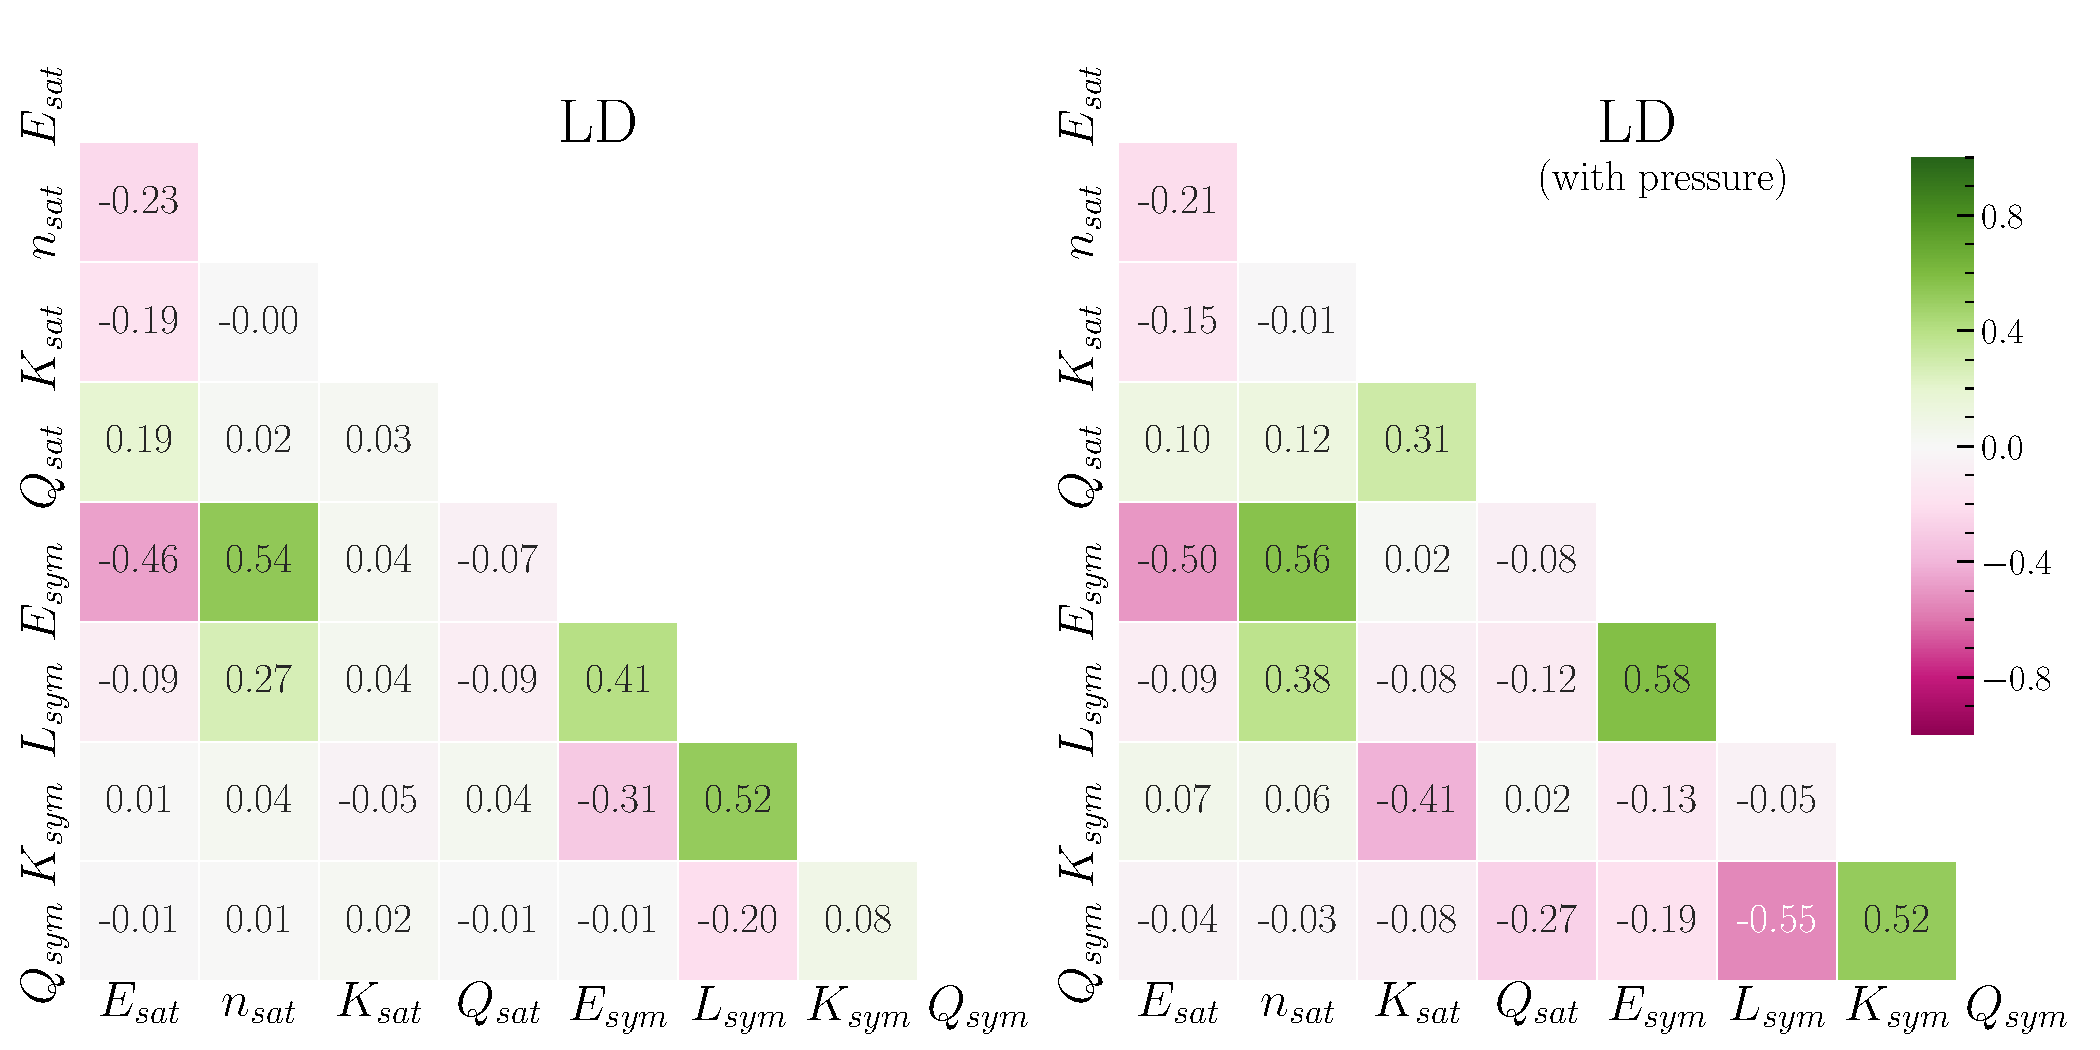
\includegraphics[width=1.0\linewidth]{figures/cm_ld.pdf}
\end{center}
\caption[Correlations among empirical parameters for the sets passing through
the low-density filter]{Correlation matrix for the empirical parameters of 
  orders $N \leq 3$ for the sets passing through the LD filter without (left) 
  and with (right) the constraint on pressure. The likelihood probability 
$p_{\text{AME2016}}$ is accounted for and $p=3$ is fixed.}\label{fig:cm_ld}
\end{figure}
 
We now turn to explore the correlations between empirical parameters, as
obtained by applying the different conditions. As in~\ref{subsubsec:marg},
$p=3$ is fixed, and the likelihood probability $p_{\text{AME2016}}$ is 
accounted for in all cases. 
Given a pair of parameters $(X_i,X_j)$, the Pearson correlation coefficient is 
calculated as 
%
\begin{equation}
  r_{ij} = \frac{\text{cov}(X_i,X_j)}{\sigma_{X_i}\sigma_{X_j}},
\end{equation}
%
where $\text{cov}(X_i,X_j)$ is the covariance and $\sigma_{X_i}$ 
($\sigma_{X_j}$) is the standard deviation of the parameter $X_i$ ($X_j$).

\begin{figure}[!t]
\begin{center}
  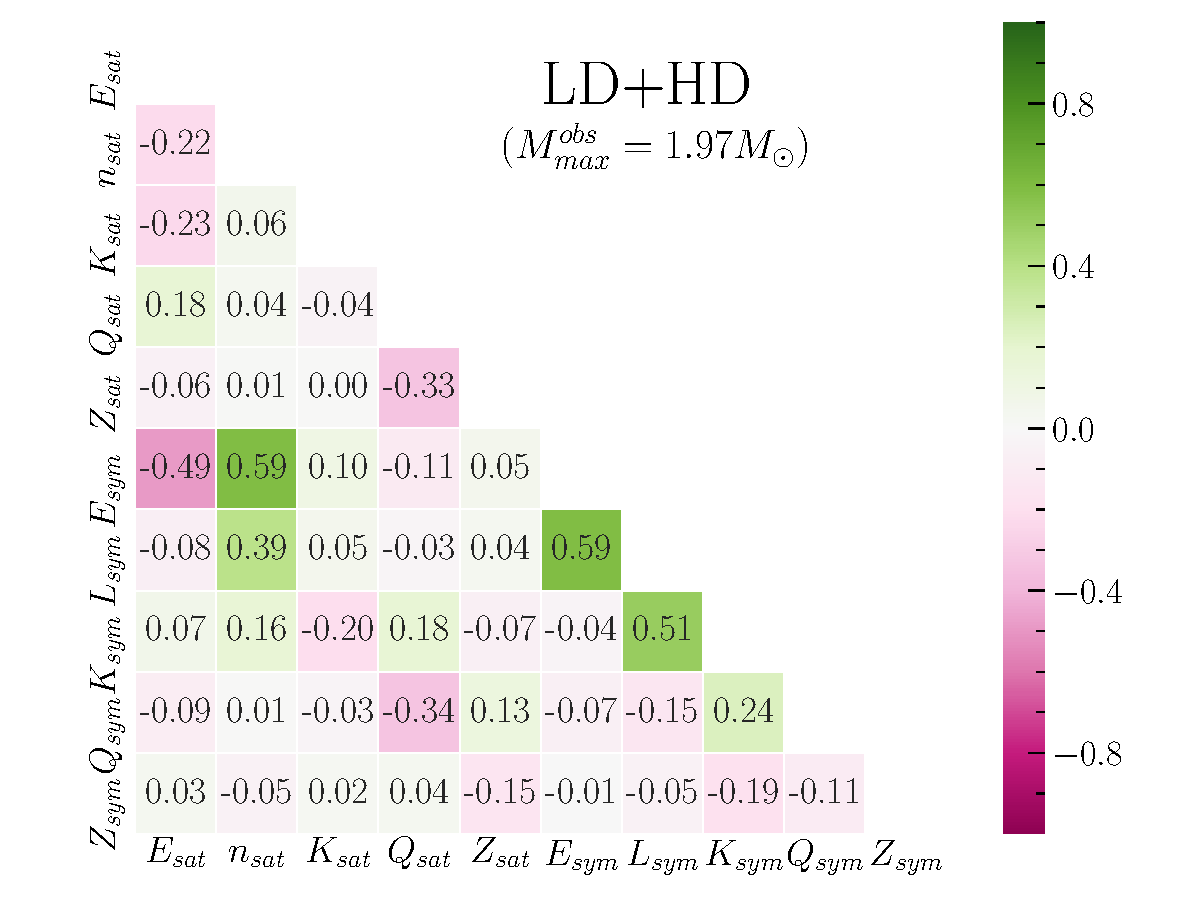
\includegraphics[width=0.9\linewidth]{figures/cm_ldhd.pdf}
\end{center}
\caption[Correlations among empirical parameters for the sets passing through
both low-density and high-density filters]{Correlation matrix for the empirical 
  parameters of orders $N \leq 4$ for the sets passing through both LD and HD 
  filters without the constraint on pressure, for 
  $M_{max}^{obs}=1.97M_\odot$~\cite{Antoniadis2013}. The likelihood probability 
$p_{\text{AME2016}}$ is accounted for and $p=3$ is fixed.}\label{fig:cm_ldhd}
\end{figure}
 
In Fig.~\ref{fig:cm_ld}, we find that many correlations appear due to the LD 
constraints. The left panel of the figure shows the correlation matrix for the 
empirical parameters of orders $N \leq 3$ for the sets passing through the LD 
filter without applying the constraint on pressure arising from chiral EFT. We 
find an anticorrelation between $E_{sat}$ and $E_{sym}$, and a positive 
correlation between $E_{sym}$ and $n_{sat}$. More interesting correlations 
among the different isovector parameters are induced by the constraint of 
reproducing the ab initio EFT calculations. Indeed, we recover the correlation 
between $E_{sym}$ and $L_{sym}$, which has been already observed by many 
authors using different models 
\cite{Lim2019tidal,Kortelainen2012,Danielewicz2014,Trippa2008,Colo2014}.
We also observe a strong correlation between $L_{sym}$ and $K_{sym}$ and find
that $E_{sym}$ is slightly anticorrelated to $K_{sym}$.

The correlation matrix calculated from the joint posterior distributions of
parameters for the sets passing through chiral EFT predicted bands both for 
energy per nucleon and pressure of NM is displayed in right panel of 
Fig.~\ref{fig:cm_ld}. Several differences with respect to the matrix in the 
left panel can be noticed.
Among the isovector parameters, it is seen that the previously found 
correlation between the slope of the symmetry energy $L_{sym}$ and the 
isovector incompressibility $K_{sym}$ disappears in favor of a strong 
correlation between $K_{sym}$ and the isovector skewness $Q_{sym}$, and an 
anticorrelation between $L_{sym}$ and $Q_{sym}$. We also observe that the 
isoscalar parameters $K_{sat}$ and $Q_{sat}$ are weakly correlated with the 
corresponding isovector ones $K_{sym}$ and $Q_{sym}$. These nontrivial 
correlations can only be revealed within the metamodeling strategy, because in 
usual functionals, such as Skyrme ones, the high-order parameters are a priori 
strongly correlated from the functional form. 

In both cases studied in Fig.~\ref{fig:cm_ld}, the fourth order parameters 
$Z_{sat}$ and $Z_{sym}$ do not show any correlation with any other parameter, 
showing their negligible influence on the density relatively close to 
saturation implied in the LD filter. Similarly, the isoscalar effective mass 
and effective mass splitting are also essentially uncorrelated 
with the others. The reason is that variations of these parameters, which play 
a crucial role in the structure of finite nuclei, are fully compensated by 
variations of the density derivatives as long as only the total energetics, 
that is kinetic plus potential, is involved~\cite{Chatterjee2017}.

Fig.~\ref{fig:cm_ldhd} shows the correlation matrix for the empirical 
parameters of orders $N \leq 4$ for the sets passing through both LD and HD 
filters without the constraint on pressure, for
$M_{max}^{obs}=1.97M_\odot$~\cite{Antoniadis2013}. One can identify the 
correlations induced by the application of HD filter by comparison with the 
left panel of Fig.~\ref{fig:cm_ld}. Doing so, we infer that the $w_{HD}$ 
pass-band filter does not induce any correlation among the 
empirical parameters, with the exception of $Q_{sat}$ being now slightly 
anticorrelated to $Q_{sym}$ and $Z_{sat}$. 
%
This can be understood from the fact that the maximum mass constraint is
essentially sensitive to the global stiffness of the EoS, and given the large 
uncertainties on the high-order parameters, a stiff EoS can be obtained with
many different combinations of $K_{sym}$, $Q_{sym}$, $Q_{sat}$, $Z_{sym}$, and
$Z_{sat}$, indicating a certain reduncancy in our parameter space with this
limited set of constraints.

\section{General predictions for neutron star observables}\label{sec:general}

This section deals with general predictions for NS observables, based on the
Bayesian analysis performed in Section~\ref{sec:bayes}. The marginalized
posterior for the observable $\mathcal{O}$,
%
\begin{equation}
  p(\mathcal{O}|\text{data}) = \left\{\prod_{i=1}^{2(N+1)+3}\int
  dX_i\right\}\mathcal{O}(\bm{X})p(\bm{X}|\text{data}),\label{eq:margobs}
\end{equation}
%
can be extracted from the joint posterior distribution of empirical parameters
$p(\bm{X}|\text{data})$, where $\mathcal{O}(\bm{X})$ is the value of the
observable $\mathcal{O}$ as obtained with the parameter set $\bm{X}$.
Our predictions for global properties of the NS are presented and confronted 
with popular models as well as with the GW170817 event in~\ref{subsec:gw17}. 
The Bayesian determination of the CC transition density and pressure is carried 
out in~\ref{subsec:cc_bayes}.
Finally, in~\ref{subsec:gli_stats}, we calculate the fraction of crust moment
of inertia for the joint posterior distribution of parameters in order to 
investigate whether \textit{the crust is enough} to explain pulsar glitches in 
the standard picture presented in~\ref{subsubsec:glitch}. 
{Some of the results presented in the following have been published
~\cite{Carreau2019cc,Carreau2019moi}.}

\subsection{Global properties: confrontation with popular models and the 
GW170817 event}\label{subsec:gw17}

A large number of EoS models, based for instance on Skyrme functionals or 
relativistic mean-field models, have been proposed in the literature over the 
years. Astrophysical observations can provide strong constraints on the
nuclear EoS  and therefore allow discriminating between the different models. 
For instance, we have seen from~\ref{subsec:masses} that the observations of 
massive pulsars require from the EoS to support $M_{max} \gtrsim
2M_\odot$~\cite{Demorest2010,Antoniadis2013,Cromartie2020}.
The recent GW170817 event, which is the first detection of GW from a 
binary NS coalescence, has provided a constraint on the NS tidal 
deformability~\cite{GWtidal,GW1,GW2}.

In the following, we calculate global properties of NS from the LD+HD joint 
posterior distribution of parameters and confront our results with popular EoS 
models as well as with the GW170817 constraints provided by the LIGO and Virgo 
collaborations.

\subsubsection{Equation of state} % 1

\begin{figure}[!t]
\begin{center}
  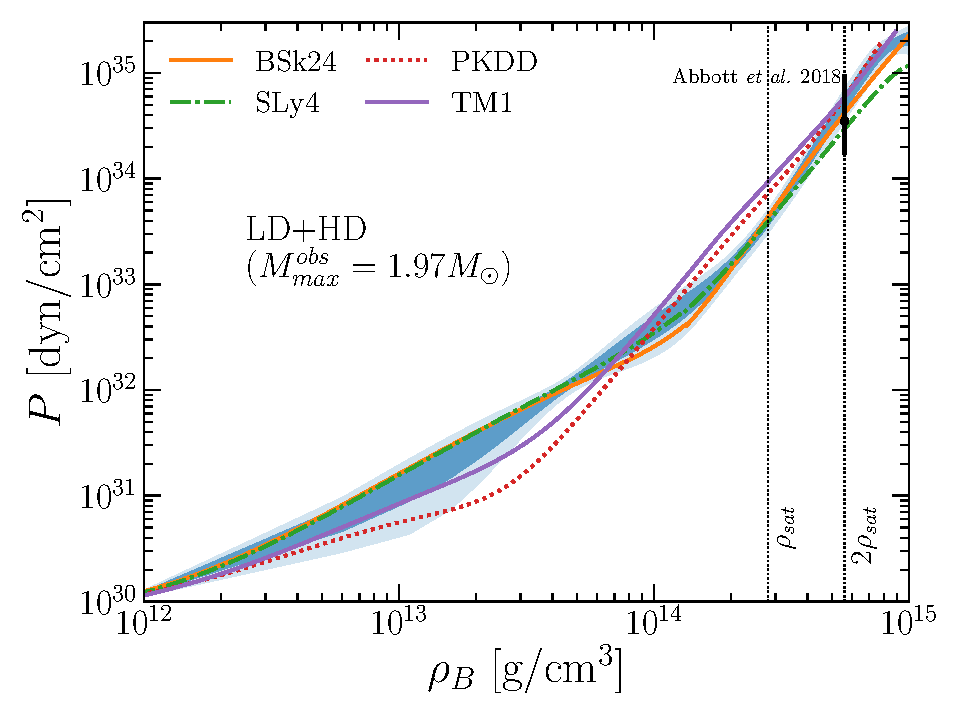
\includegraphics[width=0.9\linewidth]{figures/eos_bayes.pdf}
\end{center}
\caption[Posterior equation of state confronted with popular models and 
the GW170817 event]{Marginalized posterior for the pressure 
  $P$ as a function of the baryon mass density $\rho_B$ of the NS interior for 
  the sets passing through both LD and HD filters without the constraint on 
  pressure, for $M_{max}^{obs} = 1.97M_\odot$~\cite{Antoniadis2013}. The 
  likelihood probability $p_{\text{AME2016}}$ is accounted for and $p=3$ is 
  fixed. The blue dark and light shaded regions show the $1\sigma$ and $2\sigma$ 
  confidence intervals, respectively. The BSk24 (solid orange line), SLy4
  (dashdotted green line), PKDD (dotted red line), and TM1 (solid purple line) 
  unified EoS calculated within the metamodeling technique with $p=3$ are 
  represented. The constraint on $P_{2\rho_{sat}}$ inferred from 
  GW170817~\cite{GW1} is given.}\label{fig:eos_bayes}
\end{figure}

The $1\sigma$ and $2\sigma$ confidence regions for the posterior unified EoS,
obtained from the sets passing through both LD and HD constraints, are shown in
Fig.~\ref{fig:eos_bayes} along with four popular EoS calculated within the
metamodeling technique, namely BSk24 (solid orange line), SLy4 (dashdotted
green line), PKDD (dotted red line), and TM1 (solid purple line) EoS. 
We can see that only the EoS based on BSk24 functional is
compatible, at $2\sigma$, with the final LD+HD prediction in the whole density 
domain considered in the figure. It is observed that the SLy4 EoS deviates
below the $2\sigma$ band at suprasaturation densities.
The two EoS based on functionals issued from relativistic mean-field theory, 
namely PKDD and TM1, do not meet the final LD+HD predictions. The reason is 
that the ab initio calculations considered for our LD filter 
\cite{Drischler2016} tend to favor soft EoS, typically based on Skyrme
functionals, as we can see in Fig.~\ref{fig:iv_dist}. Indeed, we find $E_{sym}
= 30.77 \pm 1.20$ MeV and $L_{sym} = 47.11 \pm 9.54$ MeV for the low-order
isovector parameters for the LD+HD prediction, which is very close to the LD
one for these parameters. The two relativistic functionals considered
here, the empirical parameters of which are reported in
Table~\ref{table:newemppar}, exhibit a very stiff behavior at saturation.
 
The recent constraint, provided by the observation of GW170817, on 
the pressure at twice nuclear saturation density, $P_{2\rho_{sat}} =
3.5_{-1.7}^{+2.7}\times 10^{34}$ dyn/cm$^2$ at the $90\%$ level~\cite{GW1}, is 
also shown in Fig.~\ref{fig:eos_bayes}. We can see that this result is in very 
good agreement with our analysis. Let us notice that our predicted $2\sigma$ 
band at $2\rho_{sat}$ is very thin in comparison with the constraint 
arising from GW170817. This is because the ab initio calculations, not 
considered as a filter in~\cite{GW1}, impose stringent constraints on the 
low-density EoS.
%
{The excellent determination of the EoS at $2\rho_{sat}$ comes from the 
   fact that we have applied the LD constraint up to $0.20$ fm$^{-3}$. If we 
   only trust the ab initio calculations up to $\rho_{sat}$, because of the 
uncertainties on the three-body interactions that are still under
debate~\cite{Tews2019}, the prediction remains good, but the band is larger and 
compatible with the SLy4 EoS.}

\subsubsection{Masses and radii} % 1.5

\begin{figure}[!t]
\begin{center}
  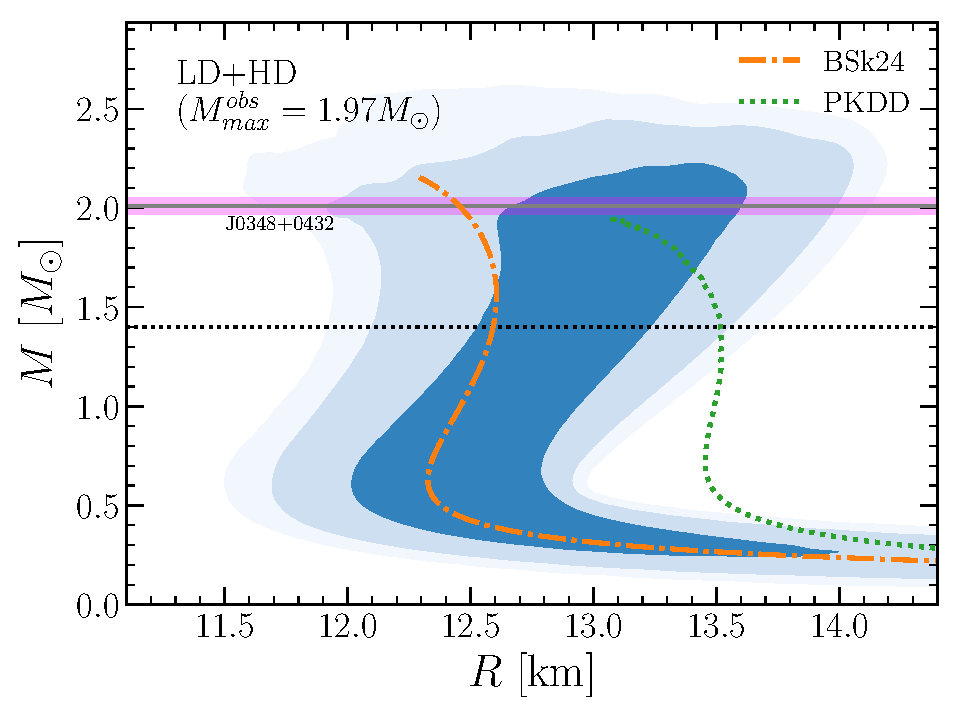
\includegraphics[width=0.9\linewidth]{figures/mr_bayes.pdf}
\end{center}
\caption[Posterior mass-radius relation confronted with popular models and 
the GW170817 event]{Marginalized posterior for the NS mass $M$ as a function of 
  the radius $R$ for the sets passing through both LD and HD filters without 
  the constraint on pressure, for $M_{max}^{obs} =
  1.97M_\odot$~\cite{Antoniadis2013} (magenta band). The likelihood 
  probability $p_{\text{AME2016}}$ is accounted for and $p=3$ is fixed. The 
  blue shaded regions show the $68\%$, $95\%$ and $99\%$ confidence 
  intervals. The mass-radius relation for the same popular EoS as in 
Fig.~\ref{fig:eos_bayes} are represented.}\label{fig:mr_bayes}
\end{figure}
 
% confrontation with popular models
In Fig.~\ref{fig:mr_bayes}, we plot the $68\%$, $95\%$ and $99\%$ 
confidence regions for the mass-radius relation obtained from the Bayesian
modeling of the EoS for the LD+HD prediction, using the marginalization 
principle, Eq.~(\ref{eq:margobs}). The mass-radius relationship for the same 
popular EoS as in Fig.~\ref{fig:eos_bayes}, namely the 
Skyrme-based BSk24 and SLy4 EoS, and relativistic PKDD and TM1 EoS, are 
represented. As we can see, only the BSk24 result (solid orange line) is 
compatible with our prediction at $95\%$ credible level in the whole mass 
domain considered. The two relativistic models predict large radii compared to 
our prediction. The soft SLy4 EoS, while similar to BSk24 EoS at low density, 
predict too small radii by $\approx 1$ km to meet the LD+HD prediction at 
$M = 2M_\odot$. Given the results presented in this figure and in
Fig.~\ref{fig:eos_bayes}, we therefore find that all known models considered 
would have been rejected by the filters except BSk24, which satisfy both LD and
HD constraints.

Let us now confront our prediction for the radius of a canonical NS,
$R_{1.4}=12.88_{-0.65}^{+0.53}$ km ($90\%$ credible interval), with different 
constraints found in the literature.
De \textit{et al.} have performed a Bayesian parameter estimation for the tidal
deformabilities and radii of NS from the observation of GW170817 within the
approximation $R_1 = R_2$, $R_1$ being the radius of the heavier star and 
$R_2$ that of the lighter star, that is assuming an identical value for the 
radius of binary components. 
The authors found $R_{1.4} = 10.7_{-1.6}^{+2.1}$ km ($90\%$ 
credible interval)~\cite{De2018}, which is in a very close agreement with the 
estimation of the LIGO/Virgo collaborations when they use EoS-insensitive 
relations, $R_{1.4} \approx R_1 = 10.7_{-1.5}^{+2.1}$ km ($90\%$ credible
interval)~\cite{GW1}. Using a parametrized EoS and imposing the constraint on
the maximum mass $M_{max}^{obs}=1.97M_\odot$, LIGO and Virgo collaborations 
further constrain $R_{1.4} \approx R_1 = 11.9_{-1.4}^{+1.4}$ km ($90\%$ 
credible interval). In all analyses, a uniform prior was used on the component 
masses. 
We find that our estimation of the canonical radius $R_{1.4}$ is 
compatible with these three analyses, even though we can notice that the our
value for the median is larger, and the $90\%$ confidence interval is 
tighter. This outlines the importance of the LD filter in our calculation, 
which ensure that our posterior is compatible with chiral EFT predicted bands 
for the energy per nucleon of SNM and PNM. Moreover, our prior distribution of 
EoS parameters contains information arising from nuclear experiments.
In~\cite{De2018,GW1}, constraints on nuclear physics observables were not 
considered.

In Fig.~\ref{fig:mr_popular}, we have observed that the study of five
characteristic EoS models suggests a possible correlation between 
the radius of the star $R$ and the slope of the symmetry energy $L_{sym}$. 
This correlation has 
been highlighted recently in several studies, using EoS based either on
Skyrme forces or relativistic mean-field models~\cite{Alam2016,Ji2019,Hu2020}. 
Surprisingly, for the LD prediction, we find that $R_{1.4}$ is especially 
correlated with the isovector incompressibility $K_{sym}$, 
$r(K_{sym},R_{1.4})=0.69$ rather than with the $L_{sym}$, 
$r(L_{sym},R_{1.4})=0.33$. As previously discussed in~\ref{subsubsec:sensana}, 
the functional forms of Skyrme forces or relativistic models generally induce 
artificial correlations between some of the empirical parameters, with the 
effect of altering true correlations. The metamodeling technique prevents this 
problem because no a priori correlation exists among the empirical parameters, 
so the true correlation are brought by the passage through LD and HD filters. 
For instance, correlations in the isovector sector between $E_{sym}$ and 
$L_{sym}$, and between $K_{sym}$ and $3E_{sym}-L_{sym}$, have been shown 
in~\cite{Mondal2017,Margueron2019} using a larger set of characteristic EoS
models.

\subsubsection{Tidal deformability} % 2

The tidal effects arising from a binary NS coalescence are encoded in the GW 
signal through the binary tidal deformability,
%
\begin{equation}
  \tilde{\Lambda} = \frac{16}{13}\frac{(m_1+12m_2)m_1^4\Lambda_1 +
  (m_2+12m_1)m_2^4\Lambda_2}{(m_1+m_2)^{1/5}},
\end{equation}
%
where $\Lambda_{1,2}$ are the individual NS tidal deformabilities,
and $m_{1,2}$ the component masses satisfying the inequality $m_1 \geq m_2$.
The binary tidal deformability is essentially correlated with the so-called
chirp mass,
%
\begin{equation}
  \mathcal{M} = \frac{(m_1 m_2)^{3/5}}{(m_1 + m_2)^{1/5}}.
\end{equation}
%
For the specific case of GW170817, this quantity has been well constrained 
to $\mathcal{M}_\text{GW170817} 
= 1.188_{-0.002}^{+0.004}M_\odot$~\cite{GWtidal}. The probability distributions 
for the component masses $m_1$ and $m_2$ are obtained from 
$\mathcal{M}_\text{GW170817}$ and the mass ratio $m_2/m_1$ (see Fig.~4
of~\cite{GWtidal}). The black dashed lines in Fig.~\ref{fig:tidal_bayes} show 
the $50\%$ and $90\%$ confidence intervals as obtained by the LIGO and Virgo 
collaborations for the low-spin prior ($|\chi| < 0.05$, $\chi$ being the
dimensionless spin), which is consistent with binary NS systems~\cite{GW2}.

\begin{figure}[!t]
\begin{center}
  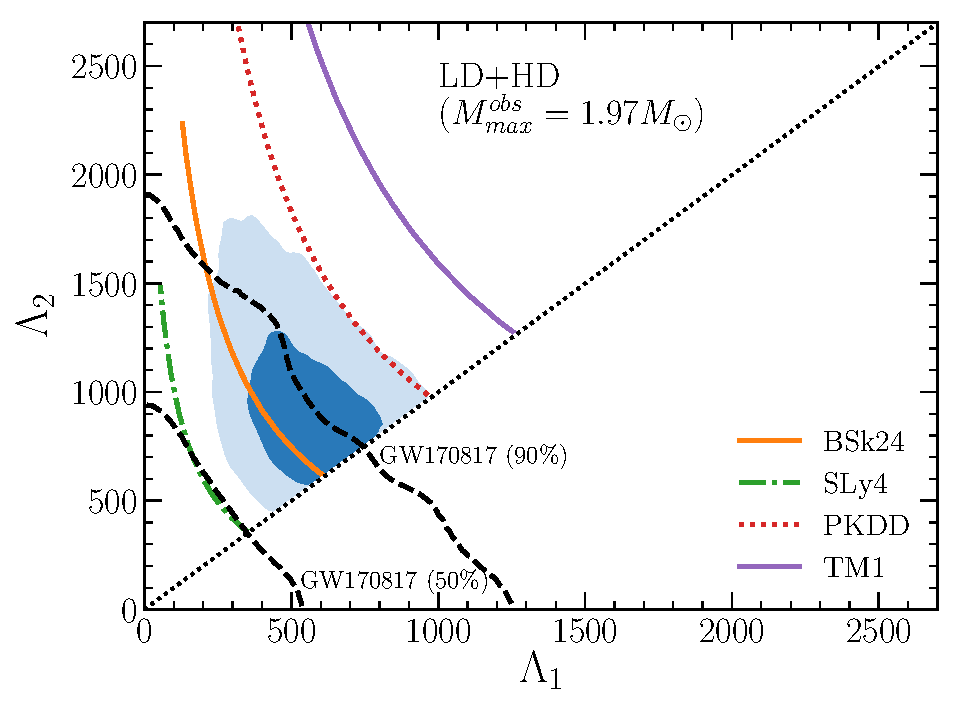
\includegraphics[width=0.9\linewidth]{figures/tidal_bayes.pdf}
\end{center}
\caption[Posterior $\Lambda_1-\Lambda_2$ relation confronted with popular 
models and the GW170817 event]{Marginalized posterior for $\Lambda_1$ (more
massive component) and $\Lambda_2$ (less massive component) for
the sets passing through both LD and HD filters without the constraint on
pressure, for $M_{max}^{obs}=1.97M_\odot$. The value of the chirp mass 
corresponds to the specific case of GW170817, $\mathcal{M} = 1.188M_\odot$, and
the individual probability distributions for $m_1$ and $m_2$ are taken
from~\cite{GWtidal}. 
Dark (light) shaded regions represents the $50\%$ ($90\%$) confidence interval 
with our Bayesian estimation with $p=3$. The black dashed lines show the $50\%$ 
and $90\%$ confidence regions as obtained by LIGO/Virgo collaborations for the 
low-spin prior~\cite{GW1}. The $\Lambda_1-\Lambda_2$ relation is also
represented for the same popular EoS as in Fig.~\ref{fig:eos_bayes}. The 
diagonal dotted line marks the $\Lambda_1=\Lambda_2$ 
boundary.}\label{fig:tidal_bayes}
\end{figure}

We show in Fig.~\ref{fig:tidal_bayes} the $50\%$ and $90\%$ confidence
regions corresponding to the joint probability distribution for $\Lambda_1$ 
and $\Lambda_2$ that we obtain for the sets passing through both LD and HD 
filters for the chirp mass $\mathcal{M}_\text{GW170817}$. The mass of the 
components have been sampled according to their respective individual 
probability distributions given in~\cite{GWtidal}, and the same EoS have been 
used to calculate the individual tidal deformabilities. The part under
the diagonal corresponds to the unphysical region $\Lambda_2 > \Lambda_1$ since 
the convention $m_1 \geq m_2$ has been taken. It is seen that our 
LD+HD prediction meets the results of the LIGO/Virgo collaborations at 
$90\%$ confidence level, but we find that our posterior slightly favors larger 
values of $\Lambda_{1,2}$, that can be obtained with stiffer EoS, associated 
to less compact NS. 
The dimensionless tidal deformabilities are also calculated for the same four 
popular EoS as in Figs.~\ref{fig:eos_bayes} and~\ref{fig:mr_bayes}.
We observe that the soft SLy4 and BSk24 EoS are in a rather good agreement with 
the analysis of the LIGO and Virgo collaborations, whereas the relativistic
models PKDD and TM1 seems very unlikely. Let us recall that yet such stiff EoS
are required in order to explain the large glitches occurring in the Vela
pulsar. Among the four popular EoS, only the one based on BSk24 functional is
compatible with the LD+HD prediction.

\begin{figure}[!t]
  \begin{center}
    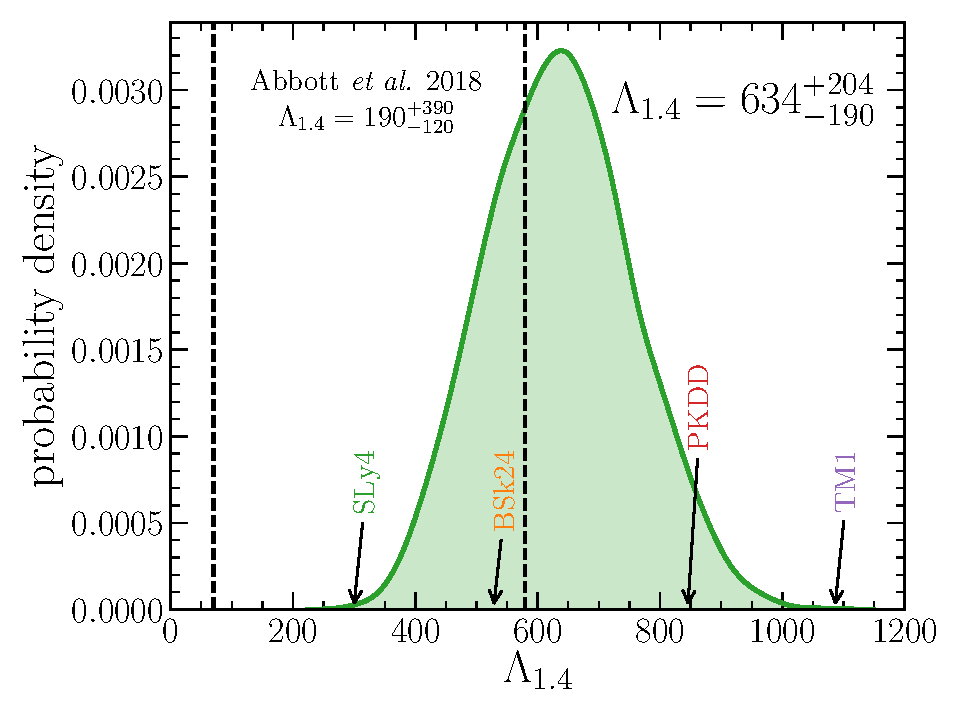
\includegraphics[width=0.9\linewidth]{figures/lambda14_bayes.pdf}
  \end{center}
  \caption[Marginalized posterior probability distribution for the 
  dimensionless tidal deformability of a $1.4M_\odot$ neutron star]{
    Marginalized posterior probability distribution for the
    dimensionless tidal deformability of a $1.4M_\odot$ NS, calculated for the 
    sets passing through both LD and HD filters without the constraint on 
    pressure, for $M_{max}^{obs}=1.97M_\odot$. The resulting $90\%$ credible 
    interval is indicated in the top right corner. The arrows give the value of 
    $\Lambda_{1.4}$ for four characteristic EoS: BSk24, SLy4, PKDD, and TM1. 
    The vertical dashed lines delimit the $90\%$ confidence interval associated 
    to the constraint of the LIGO/Virgo collaborations for GW170817, 
  $\Lambda_{1.4}=190_{-120}^{+390}$~\cite{GW1}.}\label{fig:lambda14_bayes}
\end{figure}

The marginalized posterior distribution that we obtain for the dimensionless 
tidal deformability of a $1.4M_\odot$ NS is shown in 
Fig.~\ref{fig:lambda14_bayes}, along with the prediction of characteristic EoS
based on Skyrme and relativistic models. The $90\%$ confidence interval
corresponding to the LD+HD prediction is $\Lambda_{1.4}=634_{-190}^{+204}$. It 
meets the results of the LIGO/Virgo collaborations for GW170817, 
$\Lambda_{1.4}=190_{-120}^{+390}$, the $90\%$ confidence interval of which is 
given by the vertical dashed lines in the figure. 
However, we find that the probability for $\Lambda_{1.4} < 300$ is 
negligible. The shift of the median with respect to that inferred from
GW170817 event outlines the importance of the LD filter in our calculation.
Indeed, it is known that $\Lambda_{1.4}$ is strongly correlated to the NS
radius $R_{1.4}$, we find a Pearson correlation coefficient of $r(R_{1.4},
\Lambda_{1.4})=0.98$, and we have seen that the radius of a $1.4M_\odot$ NS is 
correlated with the isovector incompressibility parameter $K_{sym}$. Hence, 
we observe that $K_{sym}$ and $\Lambda_{1.4}$ are correlated, with
$r(K_{sym},\Lambda_{1.4}) = 0.66$. We have seen in Fig.~\ref{fig:iv_dist} that 
the isovector empirical parameters are strongly constrained by the ab initio 
calculations of NM, particularly when the constraint on pressure is accounted 
for in the LD pass-band filter. More specifically, we find that the 
isovector incompressibility is tightly determined in that case, with a 
distribution being peaked at $K_{sym} \approx -200$ MeV, therefore favoring 
soft EoS and in consequence smaller values of the tidal parameter 
$\Lambda_{1.4}$.
%

{The only hypothesis of the metamodel is that the EoS can be
  written as a Taylor series, which excludes the eventuality of a first-order 
  phase transition, notably to quark-gluon plasma.
Hence, a discrepancy between our posterior and that of the
LIGO and Virgo collaborations would be a smoking gun for the existence of
quarks in the core of NS. We do not observe such evidence in the our results, 
thus the hypothesis of a purely nucleonic EoS cannot be excluded.}

\subsection{Bayesian analysis of the crust-core
transition}\label{subsec:cc_bayes}

The precise estimation of the CC transition point location, defined by
Eq.~(\ref{eq:cctp}), is important for the theoretical determination of NS 
static properties, such as the radius~\cite{Fortin2016}, for which accurate 
measurements will hopefully be available in the near future using hard x-ray 
timing techniques~\cite{Watts2016}. 
Furthermore, the computation of the crustal observables with the hydrostatic 
equilibrium equations requires the knowledge of the CC transition pressure 
$P_t$ in addition to the EoS. 
In the following, we make quantitative predictions on the density and
pressure of the CC transition point from the joint posterior distribution, and 
examine in details the influence of the different EoS parameters, as well as 
the effectiveness of the different filters entering the likelihood 
probability, Eq.~(\ref{eq:likelihood}).

\begin{figure}[!t]
  \begin{center}
    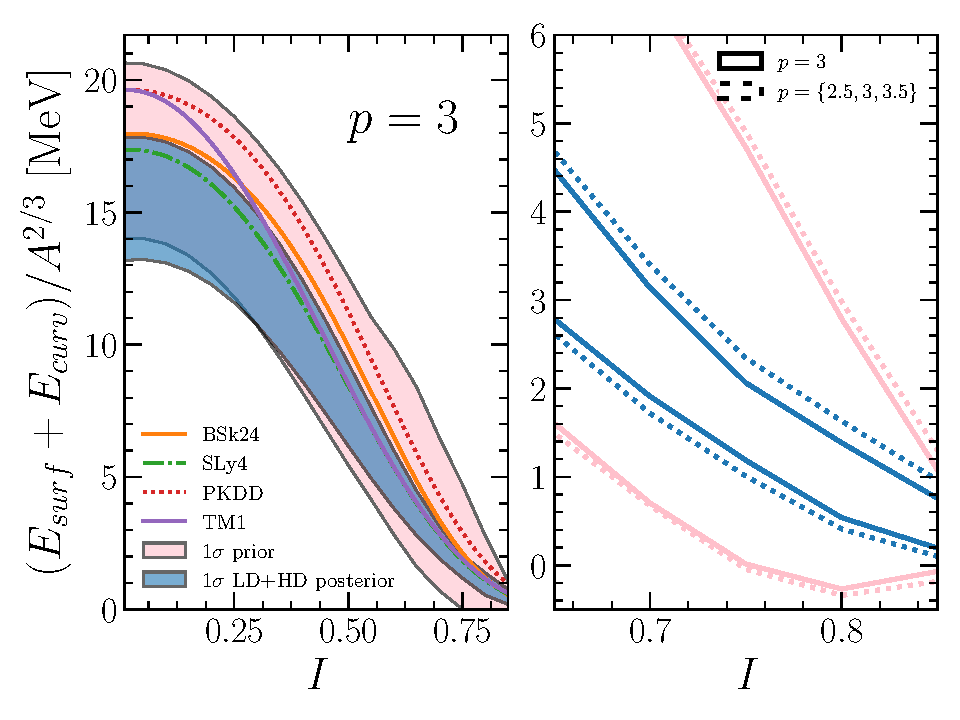
\includegraphics[width=0.9\linewidth]{figures/surf_bayes.pdf}
  \end{center}
  \caption[Prior and posterior distribution for the surface plus curvature
  energy per surface nucleon versus isospin asymmetry]{Left: $1\sigma$ prior
    (pink band) and LD+HD posterior distribution (blue band) for the surface 
    plus curvature energy per surface nucleon, defined by 
    Eqs.~(\ref{eq:esurf})-(\ref{eq:sigmac}), as a 
    function of the isospin asymmetry long the isobaric chain $A=200$ for
    $p=3$. The results for four characteristic EoS are also given. 
    Right: $1\sigma$ prior and LD+HD posterior for 
    $(E_{surf} + E_{curv})/A^{2/3}$ at high isospin for $p=3$ (solid lines) and 
  $p=\{2.5,3,3.5\}$ (dotted lines).}\label{fig:surf_bayes}
\end{figure}

% introduction surface energy
Following the strategy introduced in~\ref{subsec:ccfromc}, we calculate the CC 
transition properties from the crust, the description of which demands an
explicit modeling of clusterized matter, thus the introduction of a surface
(and eventually curvature) term in the energetics. This is done 
within the classical CLD approximation, using
Eqs.~(\ref{eq:esurf})-(\ref{eq:sigmac}). For a given set of empirical
parameters, we expect that the theoretical determination of the CC transition 
point is sensitive to the surface energy at high isospin, which is essentially 
governed by the isovector surface parameter $p$, see Fig.~\ref{fig:sly4_nt}.
Unfortunately, experimental data are unavailable above $I = (N-Z)/A \gtrsim 
0.3$, which approximately corresponds to the neutron drip line in the
laboratory.

% description prior/posterior
The prior and LD+HD posterior distribution for the
surface plus curvature energy per surface nucleon are displayed in the left 
panel of Fig.~\ref{fig:surf_bayes} as a function of isospin asymmetry for the 
$p=3$ case, along the isobaric chain $A=200$. 
%
{To obtain the prior distribution, we calculate the surface plus 
  curvature energy for the uncorrelated prior distribution of 
  empirical parameters given in Table~\ref{table:prior}. Since, for a given set
  of empirical parameters sampled according to the uniform distribution, we 
  only keep the set of surface and curvature parameters that minimizes the 
  reduces $\chi^2$ defined in Eq.~(\ref{eq:chi2}), the prior distribution 
  already takes into account the present knowledge on experimental masses.} 
%
The variation with $I$ of $(E_{surf} + E_{nuc})/A^{2/3}$ is also shown for 
four popular models. All of them are compatible with the $1\sigma$ band 
for to prior distribution.
It is seen that the LD+HD distribution predicts a lower surface energy for 
nearly symmetric nuclei with respect to the prior distribution and the 
selected popular functionals. This is not surprising because we known that the 
surface parameter $\sigma_0=\sigma(I=0)$ is strongly anticorrelated with the 
energy per nucleon of SNM at saturation $E_{sat}$~\cite{Carreau2019cc}, for 
which large values are favored by the LD filter, see Fig.~\ref{fig:is_dist}.
Above the neutron drip line, $I \gtrsim 0.35$, we can see that the filters 
defining our likelihood probability allow a tight determination of the 
surface energy in comparison to the prior distribution. This translates into
smaller uncertainties for the CC transition density and pressure.

% description p=3/p={2.5,3,3.5}
The effect of allowing a distribution for the parameter $p$ on the 
prior and LD+HD posterior distributions can be seen in the right panel of 
Fig.~\ref{fig:surf_bayes}. In spite of the simple discrete ansatz
$p=\{2.5,3,3.5\}$, we observe a continuous and smooth distribution of the
surface tension. The reason is that the variation of the surface tension 
$\sigma$ with $p$ is continuous and smooth, and that the other surface
parameters, which are fixed by the fit to experimental masses, have a
continuous distribution. The effect of allowing a distribution for the
parameter $p$ does not modify the behavior of the surface energy in the
vicinity of $I=0$. However, above the drip line and particularly in the high
isospin region, we can clearly observe that the uncertainties associated to 
the discrete ansatz are larger than those associated to $p=3$ case. 
% surprisingly, different behavior with respect to epja results
Let us notice that this effect is much more important in~\cite{Carreau2019cc}.
This can be understood from the fact that, in the latter study, curvature terms 
were not accounted for, and that the surface parameters were fitted
to the spherical magic and semimagic nuclei $^{40,48}$Ca, $^{48,58}$Ni,
$^{88}$Sr, $^{90}$Zr, $^{114,132}$Sn, and $^{208}$Pb, while the surface and 
curvature parameters are here fitted to the 2498 experimental masses of the 
AME2016~\cite{Huang2017}.

\begin{figure}[!t]
  \begin{center}
    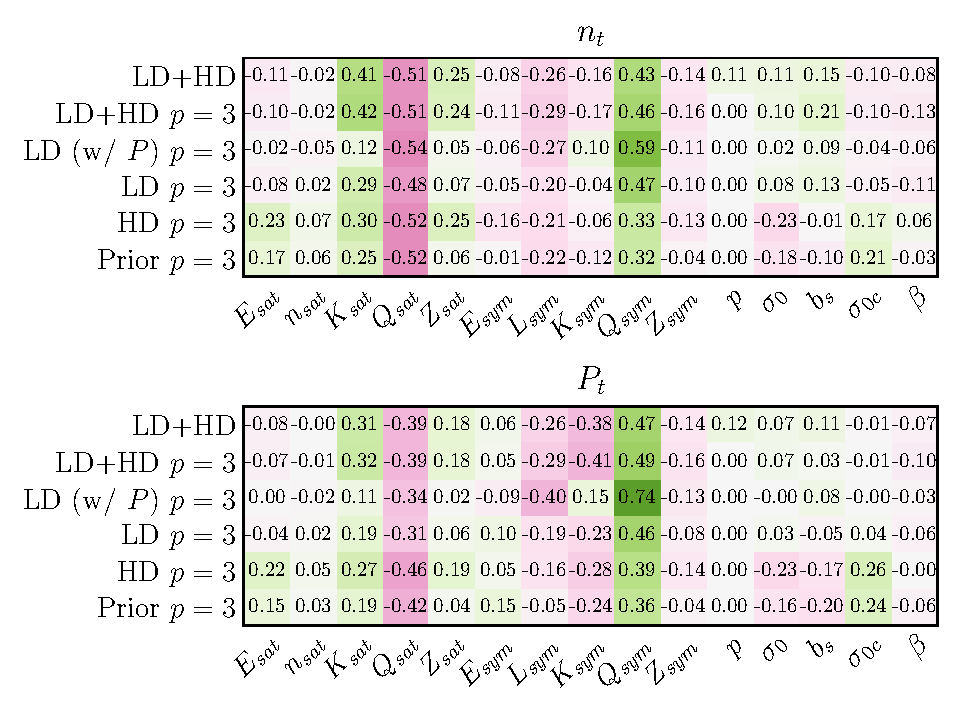
\includegraphics[width=\linewidth]{figures/corr_ntpt_pars.pdf}
  \end{center}
  \caption[Correlation of the crust-core transition density and pressure with 
  the equation of state parameters for different filters]{Correlation of the CC 
    transition 
    density $n_t$ (upper panel) and pressure $P_t$ (lower panel) with the
    empirical, surface, and curvature parameters for different distributions: 
    prior, HD, LD, LD with pressure filter, and LD+HD joint posterior 
    distributions for $p=3$, and LD+HD joint posterior distribution for the 
    discrete ansatz $p=\{2.5,3,3.5\}$.}\label{fig:corr_ntpt_pars}
\end{figure}

% intro figure
The correlation coefficients between the EoS parameters and the density and
pressure at the CC transition point are calculated and reported in 
Fig.~\ref{fig:corr_ntpt_pars} for different joint distributions of parameters.
% prior
For the prior distribution, which corresponds to the consideration of nuclear
experimental constraints included as fully uncorrelated parameters sets, we 
observe that the most influential empirical parameters on $n_t$ and $P_t$ are 
the high-order parameters $Q_{sat}$ and $Q_{sym}$.
We also recover a small anticorrelation between the transition density and the 
$L_{sym}$ parameter, as anticipated in~\ref{subsec:ccfromc}. The transition 
density directly depends on the energy of beta-equilibrated matter. The 
transition pressure being linked to the first derivative of the energy density, 
it is not surprising to observe that $P_t$ is rather slightly anticorrelated 
with $K_{sym}$. Since this parameter widely varies in existing functionals, 
this can explain why the present predictions of the transition pressure are so 
largely scattered, see Fig.~\ref{fig:cctp_lsym}.
% effects of filters
The HD filter does not impose further correlations between the transition
quantities and the EoS, apart from tiny 
correlations with the isoscalar kurtosis $Z_{sat}$. We can see that the LD 
filter slightly reinforces the correlation of transition density and pressure 
with the isovector skewness $Q_{sym}$. If the pressure filter, which allows a
tight determination of the low-order isovector parameters, is also
considered, the correlations with $Q_{sym}$ are even stronger,
$r(Q_{sym},n_t)=0.59$ and $r(Q_{sym},P_t)=0.74$. In addition, the 
anticorrelation between $L_{sym}$ and $P_t$ emerges, with 
$r(L_{sym},P_t)=-0.40$. For our final LD+HD prediction with $p=3$, we find that
$n_t$ is correlated with $K_{sat}$ and $Q_{sym}$, and anticorrelated with
$Q_{sat}$. A slight correlation with $L_{sym}$ can also be seen. Concerning the
transition pressure $P_t$, correlations with the isovector empirical parameters
$L_{sym}$, $K_{sym}$ and $Q_{sym}$ are observed, as well as with 
$K_{sat}$ and $Q_{sat}$ in the isoscalar sector.
% surface energy (all the empirical parameters are preserved)
It is seen that correlations of the transition quantities with the surface and
curvature parameters are negligible in this study, even if the isovector
surface parameter $p$ is allowed to vary (lines ``LD+HD''). This observation
contrasts with some of the results of~\cite{Carreau2019cc}, in which 
important correlations between the transition quantities and the surface
parameters were revealed. Once again, this is because the surface energy is
better controlled in the present calculation, as permitted by the introduction 
of curvature terms, supplemented by the fact that a larger pool of nuclear 
masses is used for the fit of surface and curvature parameters. 
We can say that the fact that important differences are observed with respect
to our published results, when the surface parameters are more strongly
constrained, is a confirmation of the main conclusion of our
paper~\cite{Carreau2019cc}, namely that a control on the surface energy is
mandatory to correctly predict the transition properties.

\begin{table}[!t]
\begin{center}
\begin{tabular}{ccccc} 
  \toprule
  \toprule
  & \multicolumn{2}{c}{This thesis} & 
  \multicolumn{2}{c}{\cite{Carreau2019cc}}\\
  Distribution & $n_t$ (fm$^{-3}$) & $P_t$ (MeV/fm$^3$) & $n_t$
  (fm$^{-3}$) & $P_t$ (MeV/fm$^3$)\\
  \midrule
  Prior & $0.062_{-0.036}^{+0.028}$ & $0.225_{-0.167}^{+0.379}$ & $0.078\pm
  0.040$ & $0.342\pm 0.426$\\
  HD & $0.059_{-0.029}^{+0.023}$ & $0.190_{-0.120}^{+0.232}$ & $0.076\pm 0.032$
     & $0.394\pm 0.327$\\ 
  LD & $0.073_{-0.032}^{+0.025}$ & $0.281_{-0.179}^{+0.478}$ & &\\ 
  LD (w/ $P$) & $0.068_{-0.021}^{+0.021}$ & $0.263_{-0.149}^{+0.302}$ & $0.074
  \pm 0.011$ & $0.307\pm 0.167$\\ 
  LD+HD & $0.074_{-0.033}^{+0.019}$ & 
  $0.277_{-0.168}^{+0.276}$\\ 
  LD (w/ $P$)+HD & $0.083_{-0.045}^{+0.016}$ & $0.463_{-0.338}^{+0.262}$ & 
  $0.077\pm 0.010$ & $0.389\pm 0.111$\\ 
  \bottomrule
  \bottomrule
\end{tabular}
\end{center}
\caption[$68\%$ confidence intervals for the crust-core transition density and
pressure for different filters]{$68\%$ confidence intervals for the CC
transition density $n_t$ and pressure $P_t$ for different distributions: prior, 
HD, LD with and without the pressure filter, {and LD+HD with and without 
the pressure filter.} In all cases, $p=3$ is fixed. {The right two columns 
give the average value and standard deviation $\sigma$ of $n_t$ and $P_t$
calculated in~\cite{Carreau2019cc}.}}\label{table:ntpt}
\end{table}

\begin{figure}[!t]
  \begin{center}
    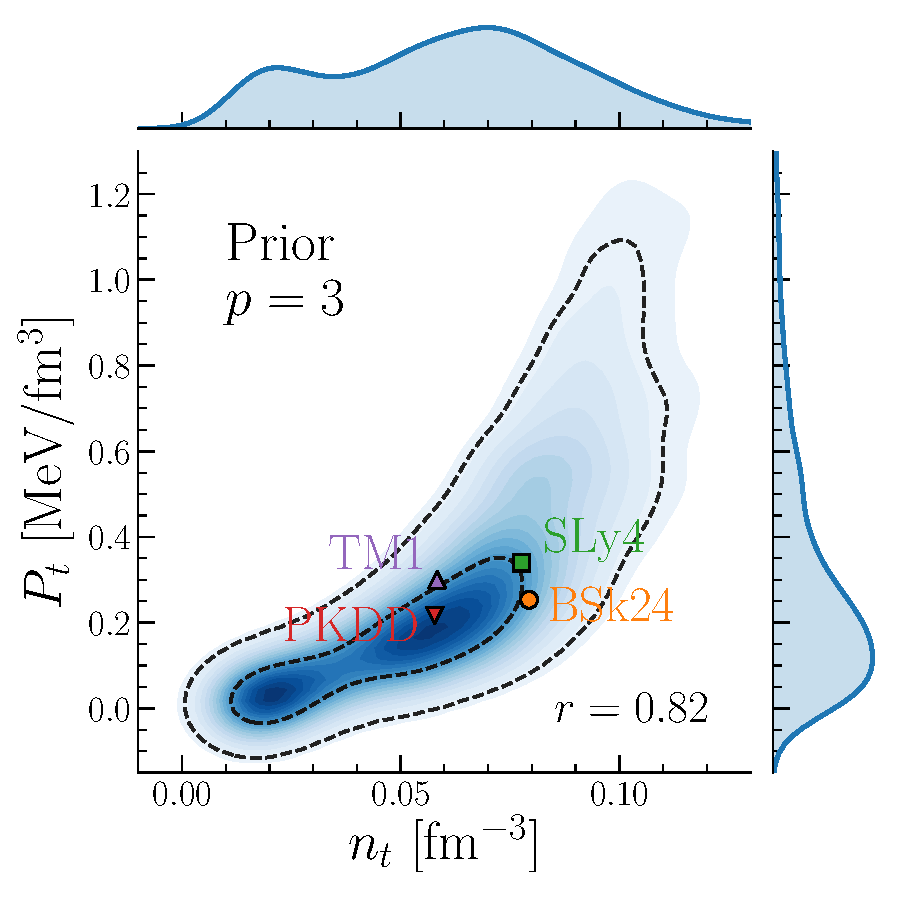
\includegraphics[width=0.42\linewidth]{figures/ntpt_priorp3.pdf}
    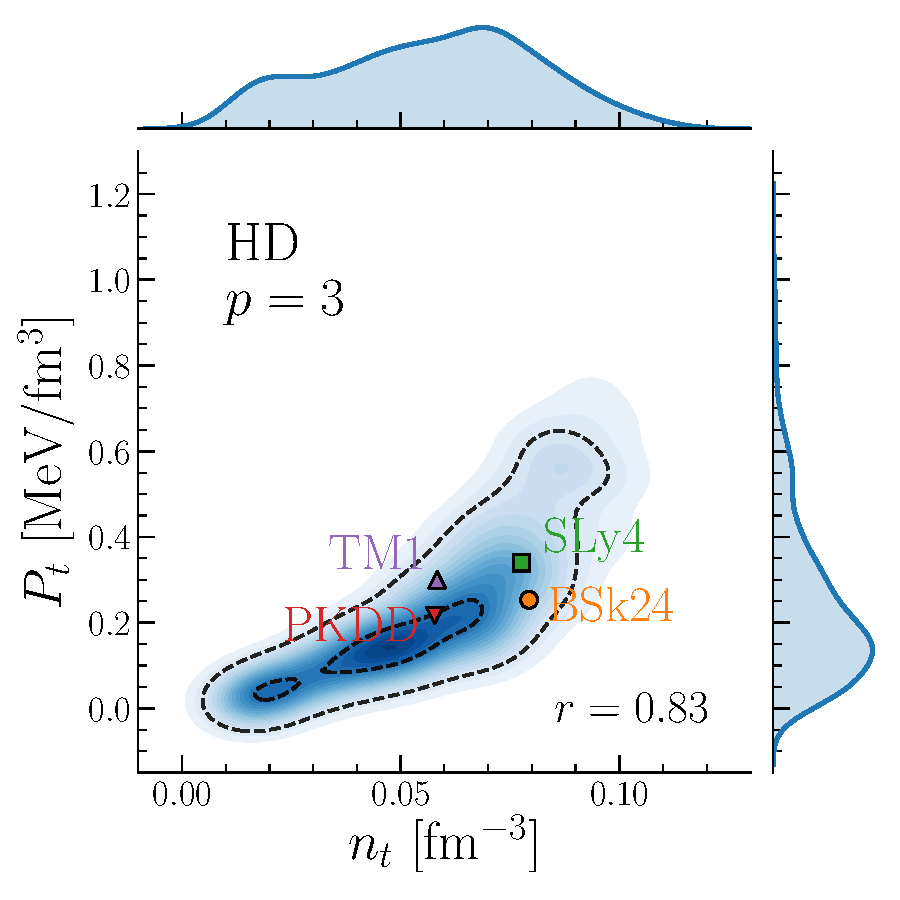
\includegraphics[width=0.42\linewidth]{figures/ntpt_hdp3.pdf}\\
    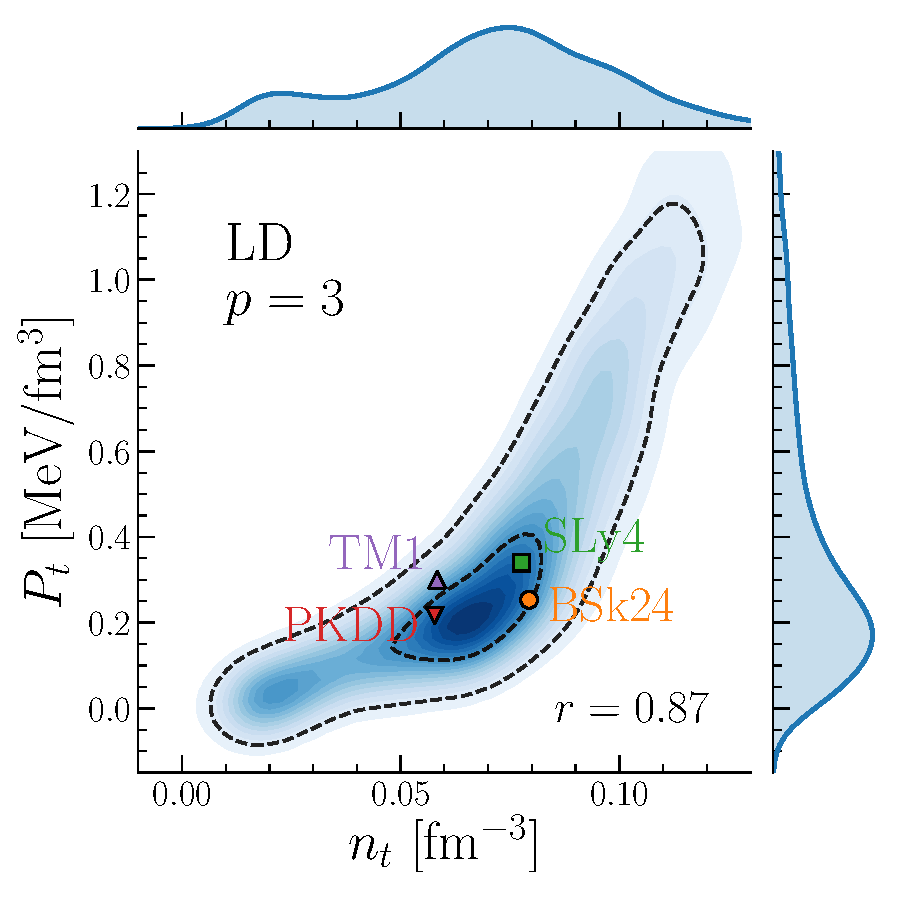
\includegraphics[width=0.42\linewidth]{figures/ntpt_ldp3.pdf}
    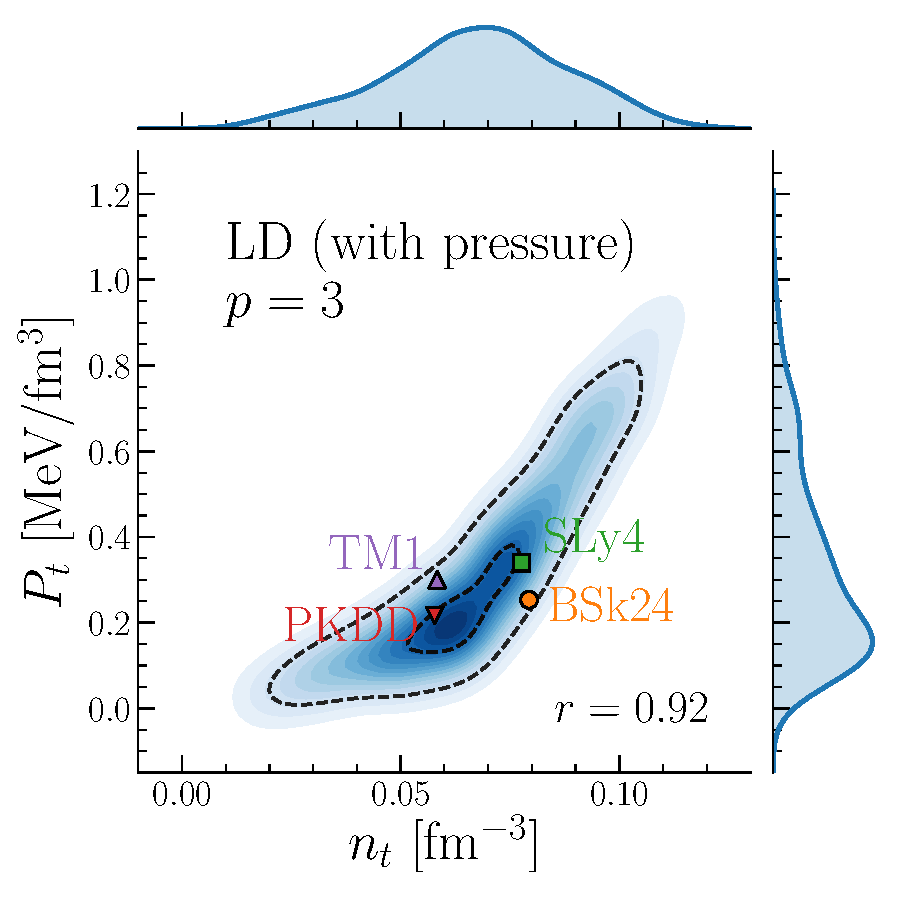
\includegraphics[width=0.42\linewidth]{figures/ntpt_ldwpresp3.pdf}\\
    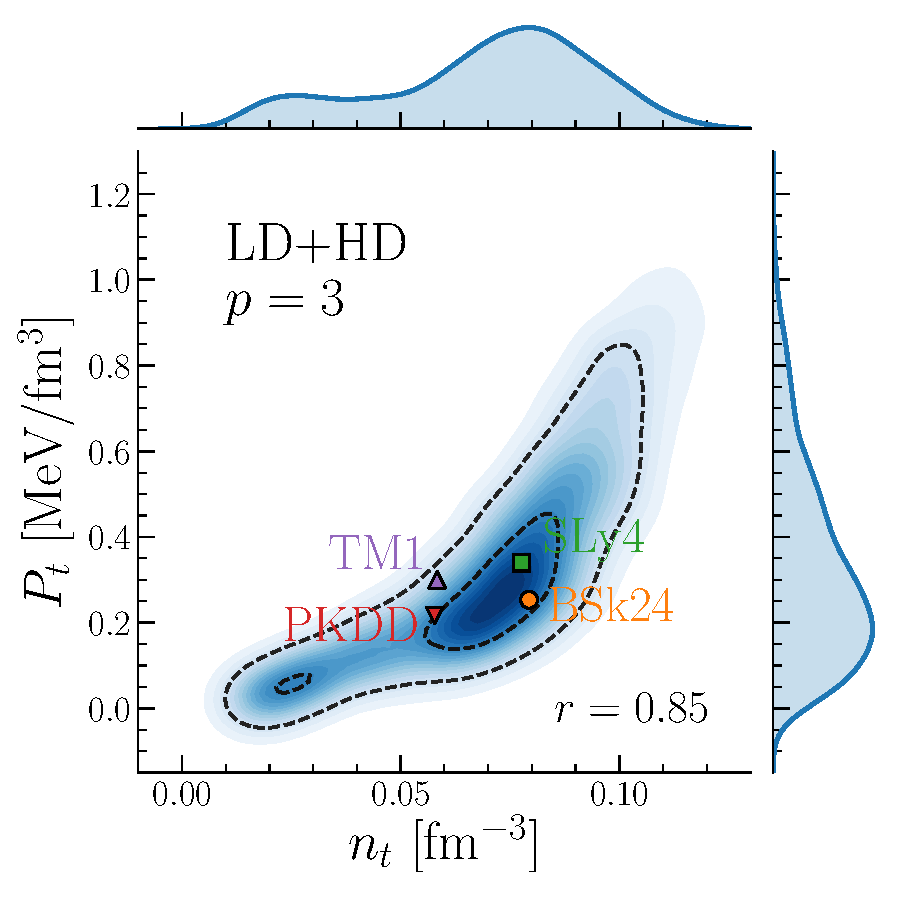
\includegraphics[width=0.42\linewidth]{figures/ntpt_ldhdp3.pdf}
    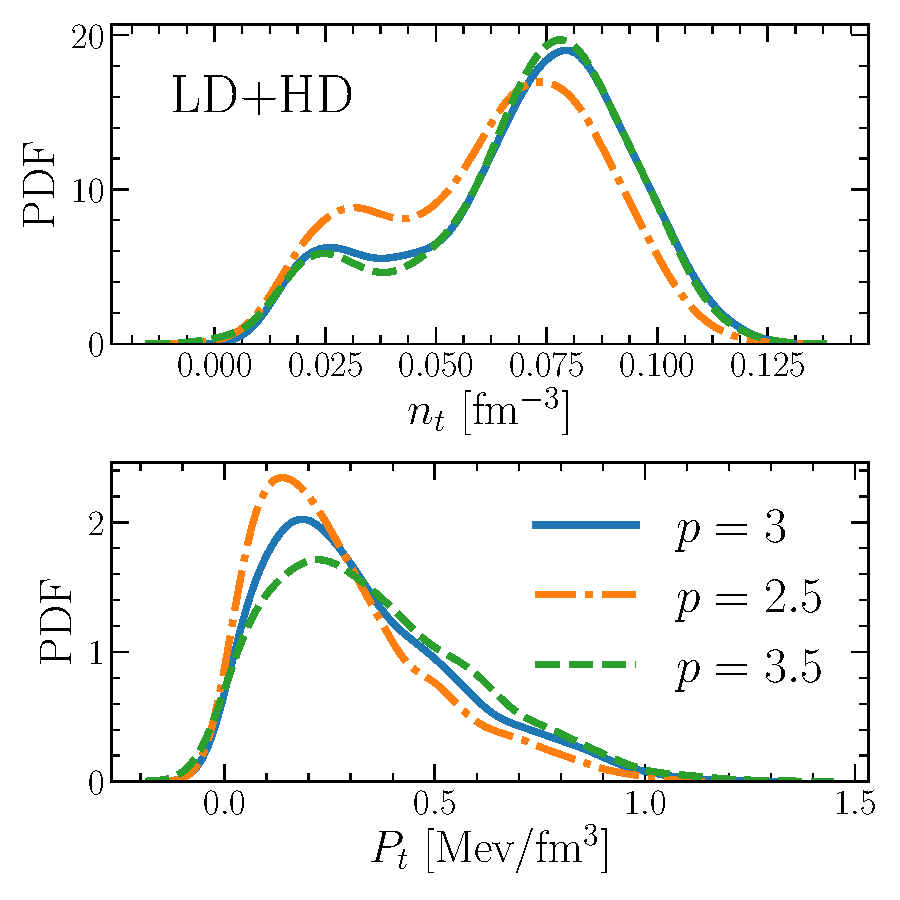
\includegraphics[width=0.42\linewidth]{figures/ntpt_marg.pdf}
  \end{center}
  \caption[Marginalized probability distributions for the crust-core transition 
  density and pressure for different filters]{Marginalized probabilities for 
    the transition density $n_t$ and pressure $P_t$ for different 
    distributions. In the first five panels, the dashed lines delimit the 
    $50\%$ and $90\%$ confidence regions. For each distribution, the Pearson 
    correlation coefficient $r(n_t,P_t)$ is given. The results for four 
    characteristic EoS are also shown.}\label{fig:ntpt}
\end{figure}

% intro figure
The joint distribution for $n_t$ and $P_t$ as well as the corresponding 
marginalized one-parameter probability distributions are shown in 
Fig.~\ref{fig:ntpt} for different filters. In the first five panels, the dashed
lines delimit the $50\%$ and $90\%$ confidence regions, and the different 
symbols give the CC transition point as obtained with the popular models BSk24, 
SLy4, PKDD and TM1. 
% strong correlation (nt,Pt) in all cases
In all cases and in agreement with~\cite{Carreau2019cc}, we find that $n_t$ and 
$P_t$ are strongly correlated. The Pearson correlation coefficient 
is as high as $r=0.92$ when using the LD filter with the constraint on 
pressure.
% Effect on the different filters on the cc transition properties / table ntpt
We can observe in a graphical way that the LD and HD constraints lead to 
compatible predictions for the CC transition point. It is clearly seen that the 
most constraining filter for both $n_t$ and $P_t$ is the LD filter which 
account for the constraint on pressure (``LD (with pressure)''), ensuring the 
compatibility of the empirical parameters with the chiral ETF predicted 
bands for energy per nucleon and pressure of SNM and PNM~\cite{Drischler2016}.
From the corresponding joint distribution, we obtain 
$n_t = 0.068_{-0.021}^{+0.021}$ fm$^{-3}$ and $P_t = 0.263_{-0.149}^{+0.302}$ 
MeV/fm$^3$ at the $1\sigma$ confidence level. The passage through the HD filter 
has a significant impact on the distribution of $P_t$. 
We find that the resulting CC transition points, for three of the four popular 
models considered in this study, meet our final LD+HD prediction at the $50\%$
confidence level.

% table
The $68\%$ confidence intervals for 
the transition density and pressure for each of the considered distributions 
{as well as for LD+HD with the pressure filter} are reported in 
Table~\ref{table:ntpt}. 
{For each filter, our predictions for $n_t$ and $P_t$ are compatible with 
our published results reported in the right two 
columns~\cite{Carreau2019cc}, though not identical due to 
a different treatment of the surface energy. Indeed, a limited pool of nine 
magic and semimagic nuclei were used to fit the surface parameters
in~\cite{Carreau2019cc}, whereas the surface and curvature parameters are
fitted to all experimental masses from AME2016 (2353 nuclei) in the present 
study. Both options have limitations. On the one hand, fitting all presently
measured masses and considering a curvature term allows a better reproduction
of experimental masses and a tighter determination of the surface parameters.
On the other hand, we fit a spherical model to nonspherical nuclei and we thus
take the risk to incorporate deformation energy components in the surface 
energy.
The fact that changing the fitting protocol of the surface and curvature
parameters alters sensitively the predictions of the transition density and
pressure means that the surface energy is a key quantity (together with the
high-order empirical parameters that are strongly constrained by the pressure 
filter), and that further investigations are desirable. In particular, a fit of 
the experimental masses with a deformation degree of freedom and shell effects, 
and an improved control of the uncertainty on pressure are advisable.
% blabla nongaussianity of the distribution in epja
Let us remark that in~\cite{Carreau2019cc}, we limited us to the calculation of 
the standard deviation for $n_t$ and $P_t$.
However, in the present study, and especially for the LD+HD prediction, 
we observe that the $68\%$ credible interval for $n_t$ and $P_t$ deviates from 
the standard deviation ($\sigma_{n_t} = 0.024$ fm$^{-3}$ and $\sigma_{P_t} = 
0.224$ MeV/fm$^3$) because of the non-Gaussianity of the distributions arising 
from the tension between LD and HD constraints observed in Fig.~\ref{fig:ntpt}.
}

% effect of varying p
The effect of varying $p$ on the marginalized one-parameter distributions for
$n_t$ and $P_t$ is displayed in the last panel of Fig.~\ref{fig:ntpt}, for the
LD+HD prediction. Overall, only minor differences are observed between the 
$p=2.5$, $p=3$ and $p=3.5$ cases. We can see that the difference between the 
$p=3$ and $p=3.5$ cases is even smaller than that between 
$p=2.5$ and $p=3$ as far as the transition density was concerned, as it was 
expected from Fig.~\ref{fig:sly4_nt}. 
%
In~\cite{Carreau2019cc}, we suggested that extra data on neutron rich nuclei
are needed to pin down the value of $p$, and consequently the transition point.
The present study suggests that an accurate reproduction of the whole pool of
presently measured masses might be sufficient to compensate the uncertainty led
by the poorly constrained $p$ parameter.

\subsection{Pulsar glitches: answering the question
``\textit{Is the crust enough?}''}\label{subsec:gli_stats}

For a given EoS, the determination of the fractional crust moment of inertia,
using Eq.~(\ref{eq:crustmoi}), 
and more generally of any crustal observable, is possible if 
the location of the transition point to homogeneous matter is known.
As discussed in~\ref{subsubsec:glitch}, the NS crustal moment of inertia is
related to the theoretical description of the glitch phenomenon, which consists
of the sudden spin-up of the rotational frequency of an NS. In the standard 
interpretation, a pulsar glitch is observed as the consequence of the angular 
momentum transfer from the neutron superfluid permeating the inner crust to the 
solid crust~\cite{Anderson1975}. For a specific pulsar for which the coupling 
parameter $\mathcal{G}$ has been measured, and depending of the importance of 
the crustal entrainment effect~\cite{Chamel2013}, the crust must therefore be 
sufficiently thick to store enough angular momentum. Naturally, it yields the 
question ``\textit{Is the crust enough?}'', for which the answer is known to be 
very sensitive to the EoS~\cite{Andersson2012,Piekarewicz2014} and, most 
important to the CC transition density and pressure~\cite{Carreau2019moi}. In 
the following, the crustal origin of pulsar glitches is discussed for the 
specific case of Vela, using the LD+HD joint posterior distribution of EoS 
parameters.

\begin{figure}[!t]
  \begin{center}
    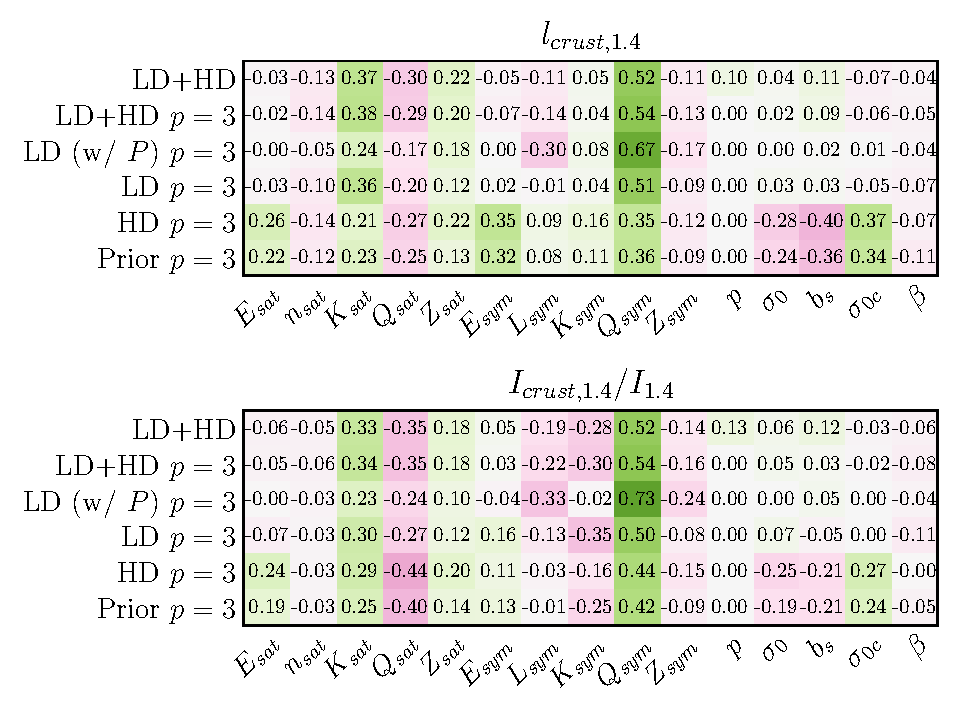
\includegraphics[width=\linewidth]{figures/corr_crustobs_pars.pdf}
  \end{center}
  \caption[{Correlation of the crust thickness and fractional crust moment 
    of inertia of a $1.4M_\odot$ neutron star with the equation of state 
    parameters for different filters}]{{Correlation of the crust thickness 
    $l_{crust,1.4}$ (upper panel) and fractional crust moment of inertia
    $I_{crust,1.4}/I_{1.4}$ (lower panel) of a $1.4M_\odot$ NS with the
    empirical, surface, and curvature parameters for different distributions: 
    prior, HD, LD, LD with pressure filter, and LD+HD joint posterior 
    distributions for $p=3$, and LD+HD joint posterior distribution for the 
drscrete ansatz $p=\{2.5,3,3.5\}$.}}\label{fig:corr_crustobs_pars}
\end{figure}
%
{
The correlation coefficients between the EoS parameters and the crust thickness
and fractional crust moment of inertia of a $1.4M_\odot$ NS are displayed in
Fig.~\ref{fig:corr_crustobs_pars} for different joint distributions of 
parameters. In agreement with our published results~\cite{Carreau2019moi}, we 
find that $l_{crust,1.4}$ and $I_{crust,1.4}/I_{1.4}$ are strongly correlated 
with the isovector skewness $Q_{sym}$. A small correlation is also obtained
between the fractional crust moment of inertia and the isovector
incompressibility $K_{sym}$. Therefore, the conclusion drawn 
in~\cite{Carreau2019moi}, that higher precision in the experimental 
determination of $K_{sym}$ and $Q_{sym}$ in the 
low density EFT theoretical predictions is required to reduce the uncertainties 
on crustal observables, clearly holds despite the different fitting protocol 
employed in the present study. 
Interestingly, as observed in Fig.~\ref{fig:corr_ntpt_pars} for 
the CC transition density and pressure, we can see that the correlations with 
the surface and curvature parameters that we observed in~\cite{Carreau2019moi} 
disappear when a refined control of the surface energy is considered.
}

\begin{table}[!t]
\begin{center}
\begin{tabular}{ccccc} 
  \toprule
  \toprule
  & \multicolumn{2}{c}{This thesis} & 
  \multicolumn{2}{c}{\cite{Carreau2019moi}}\\
  Distribution & $l_{crust,1.4}$ (km) & $I_{crust,1.4}/I_{1.4}$ ($\%$) &
  $l_{crust,1.4}$ (km) & $I_{crust,1.4}/I_{1.4}$ ($\%$)\\
  \midrule
  Prior & $1.06_{-0.33}^{+0.25}$ & $2.33_{-1.69}^{+3.37}$ & $1.13\pm 0.29$ &
  $3.40\pm 3.34$\\
  HD & $1.10_{-0.24}^{+0.21}$ & $2.20_{-1.35}^{+2.32}$ & $1.17\pm 0.29$ &
  $4.39\pm 3.26$\\ 
  LD & $1.08_{-0.27}^{+0.19}$ & $3.06_{-2.08}^{+3.65}$ & &\\ 
  LD (w/ $P$) & $0.98_{-0.20}^{+0.21}$ & $2.99_{-1.87}^{+2.65}$ & 
  $0.95\pm 0.11$ & $3.54\pm 1.33$\\ 
  LD+HD & $1.11_{-0.21}^{+0.14}$ & $2.89_{-1.68}^{+2.51}$ & &\\ 
  LD (w/ $P$)+HD & $1.10_{-0.25}^{+0.15}$ & $4.16_{-2.90}^{+2.20}$ & $1.03\pm
  0.10$ & $4.50\pm 1.25$\\ 
  \bottomrule
  \bottomrule
\end{tabular}
\end{center}
\caption[{$68\%$ confidence intervals for the crust thickness and
fractional crust moment of inertia of $1.4M_\odot$ neutron star for different 
filters}]{{$68\%$ confidence intervals for the crust thickness and 
  fractional crust moment of inertia of a $1.4M_\odot$ NS for different 
  distributions: prior, HD, LD with and without the pressure filter, and LD+HD 
  with and without the pressure filter. In all cases, $p=3$ is fixed. The right 
  two columns give the average value and standard deviation $\sigma$ of
  $l_{crust,1.4}$ and $I_{crust,1.4}/I_{1.4}$ calculated 
  in~\cite{Carreau2019moi}.}}\label{table:crustobs}
\end{table}
%
{
The $68\%$ confidence intervals for the crust thickness and fractional crust 
moment of inertia of a $1.4M_\odot$ NS are reported in 
Table~\ref{table:crustobs}. As for the transition density and pressure, we can 
see that the present predictions and our published 
results~\cite{Carreau2019moi}, reported in the right two columns, are 
compatible within error bars, but again are not identical due to a different 
treatment for the surface energy. 
Combined with the HD filter, the incorporation of the pressure filter into the 
likelihood probability has the effect of strongly increasing the value of 
$I_{crust,1.4}/I_{1.4}$. This can be observed by comparing the results 
presented in the bottom two rows.}

\begin{figure}[!t]
  \begin{center}
    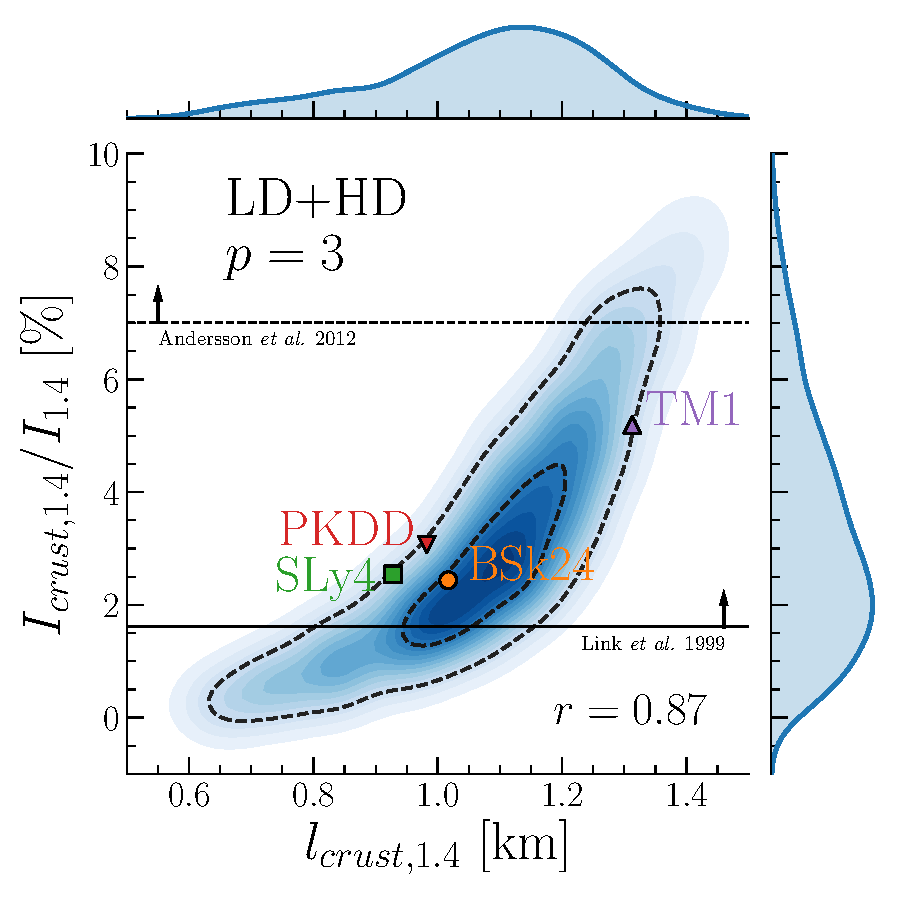
\includegraphics[width=0.8\linewidth]{figures/ifrac14_vs_lcrust14.pdf}
  \end{center}
  \caption[Marginalized probabilities for the crust thickness and fraction of
  crust moment of inertia of a $1.4M_\odot$ neutron star]{Marginalized 
    probabilities for the crust thickness $l_{crust,1.4}$ and fraction of crust 
    moment of inertia $I_{crust,1.4}/I_{1.4}$ for a $1.4M_\odot$ NS, using the 
    LD+HD distribution. The dashed lines delimit the $50\%$ and $90\%$ 
    confidence regions. The Pearson correlation coefficient $r$ is given. The 
    symbols show the prediction of four characteristic EoS 
    models. The minimum values needed to justify Vela glitches with (Andersson 
    \textit{et al.}~\cite{Andersson2012}) and without (Link \textit{et
  al.}~\cite{Link1999}) crustal entrainment are 
represented.}\label{fig:ifrac14_vs_lcrust14}
\end{figure}

The strong correlation between the crust thickness and the fraction of crust 
moment of inertia for $M=1.4M_\odot$ is seen in
Fig.~\ref{fig:ifrac14_vs_lcrust14}. It means that the thicker the crust is, 
the more angular momentum is confined to the neutron superfluid coexisting with 
the crystal lattice of the inner crust. 
As expected from previous studies~\cite{Piekarewicz2014,Carreau2019moi}, we 
observe large correlations between the crustal observables and the transition 
quantities, notably $r(P_t,I_{crust,1.4}/I_{1.4})=0.98$. Among the four popular 
models considered, only the prediction of the BSk24 EoS (orange circle) meets 
our distribution. The results for SLy4 (green square), PKDD (red triangle) and 
TM1 (purple triangle) EoS are only marginally compatible with the LD+HD 
prediction at the $90\%$ confidence level (dashed lines).
%
We can see that a crustal origin for the glitches, if the Vela pulsar has the
canonical $1.4M_\odot$ mass, appears marginal but still cannot be excluded at
the $90\%$ level, even if entrainment is accounted for (horizontal dashed
line).

\begin{figure}[!t]
  \begin{center}
    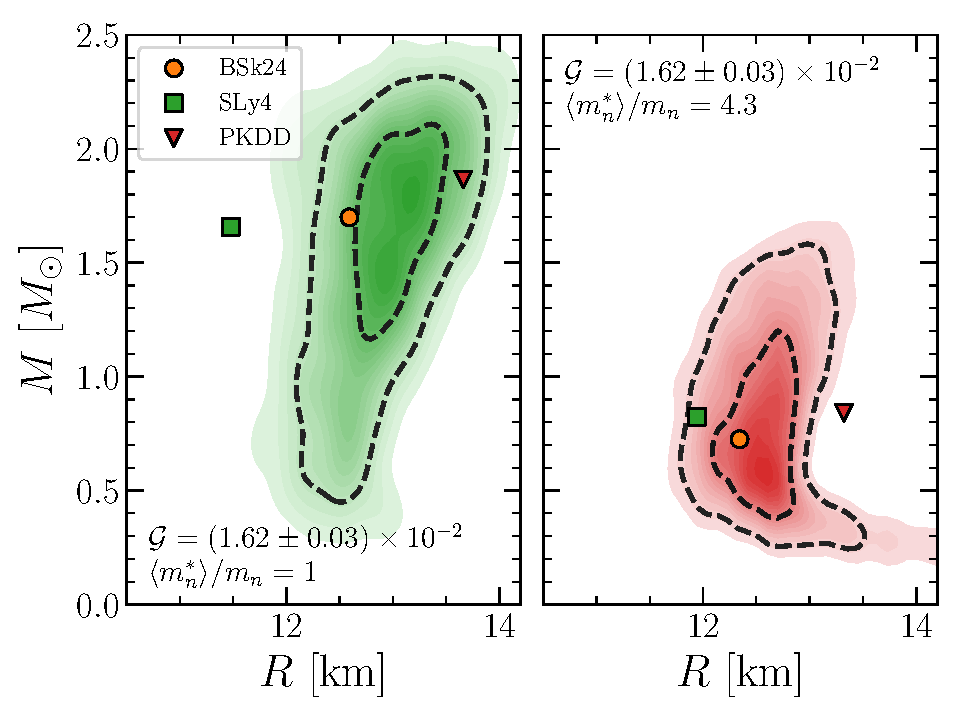
\includegraphics[width=0.9\linewidth]{figures/mr_from_g_vela.pdf}
  \end{center}
  \caption[Marginalized posterior for the neutron star mass and radius of 
  Vela]{Marginalized posterior for the NS mass $M$ and radius $R$
    of Vela, $\mathcal{G}=(1.62\pm 0.03)\times 10^{-2}$, without 
    ($\langle m_n^*\rangle/m_n = 1$~\cite{Link1999}, left panel) and with an 
    estimation of crustal entrainment ($\langle m_n^*\rangle/m_n
    =4.3$~\cite{Andersson2012}, right panel), using the LD+HD filter for 
    $p=3$. Dashed lines represent the $50\%$ and $90\%$ confidence intervals, 
    and symbols show the prediction of characteristic EoS 
  models.}\label{fig:mr_from_g_vela}
\end{figure}

From pulsar timing techniques, it is possible to infer the coupling parameter 
$\mathcal{G}$ of a given pulsar. This parameter is related to the fraction
of crust moment of inertia via Eq.~(\ref{eq:ifrac_g}). In the specific case of 
the Vela pulsar (PSR B0833-45), the coupling parameter is very well 
constrained thanks to its long-term monitoring, 
$\mathcal{G}_{\text{Vela}}=(1.62\pm 0.03)\times 10^{-2}$~\cite{Ho2015}.
Fig.~\ref{fig:mr_from_g_vela} displays the marginalized posterior distributions
for the mass and radius of Vela for two estimations of crustal entrainment,
using our LD+HD distribution.
Let us recall that the importance of the crustal entrainment effect is encoded 
in the neutron effective mass. Here, we consider $\langle m_n^* \rangle/m_n 
= 1$, that is no entrainment~\cite{Link1999}, and 
$\langle m_n^*\rangle/m_n = 4.3$, which is an estimation of crustal
entrainment~\cite{Andersson2012}. 
In this calculation, we assume that the observed glitches correspond to the 
maximum amplitude that can be sustained by the crust reservoir, which means 
that we impose the equality
%
\begin{equation}
  \frac{I_{crust}}{I} = \mathcal{G}_{\text{Vela}}\frac{\langle
  m_n^*\rangle}{m_n}.\label{eq:mr_from_g}
\end{equation}
%
Since the fractional moment of inertia is a decreasing function of the pulsar
mass, see lower panel of Fig.~\ref{fig:moi_popular}, this means that the masses 
predicted in Fig.~\ref{fig:mr_from_g_vela} should be considered as upper limits 
of the mass. 
Hence, the marginalized two-parameter distribution for Vela mass and radius is 
computed as
%
\begin{equation}
  p(M,R|\text{data})=
  \sum_{\bm{X}}\delta(M(\bm{X})-M)\delta(R(\bm{X})-R)
  p(\bm{X}|\text{data}),
\end{equation}
%
where $M(\bm{X})$ and $R(\bm{X})$ are the mass and radius obtained with the
parameter set $\bm{X}$ when the central density is such that the corresponding
fractional moment of inertia verifies Eq.~(\ref{eq:mr_from_g}). 
The resulting distribution for Vela mass and radius without entrainment (left
panel) is compatible with the uncertainties reported in Table 2 
of~\cite{Ho2015}. Evidently, the uncertainties are larger in our work since we 
consider a distribution of models, while three specific EoS (BSk20, BSk21, and 
APR) were used in~\cite{Ho2015}. In the same spirit, we show the prediction of 
BSk24, SLy4, and PKDD EoS. Considering the specific treatment of the
entrainment effect with $\langle m_n^*\rangle/m_n = 4.3$ (right panel), the 
predicted Vela mass is significantly lower than that inferred in the case where
entrainment is neglected, with $M_{\text{Vela}}=0.79_{-0.33}^{+0.41} M_\odot$ 
at the $1\sigma$ confidence level. This shows that a proper treatment of 
crustal entrainment is more important than the EoS uncertainty and the
experimental uncertainty on the glitch amplitude.
Let us notice that an innovative method was recently proposed to determine the 
mass and radius using observations of the maximum observed
glitches~\cite{Pizzochero2017}.

\begin{figure}[!t]
  \begin{center}
    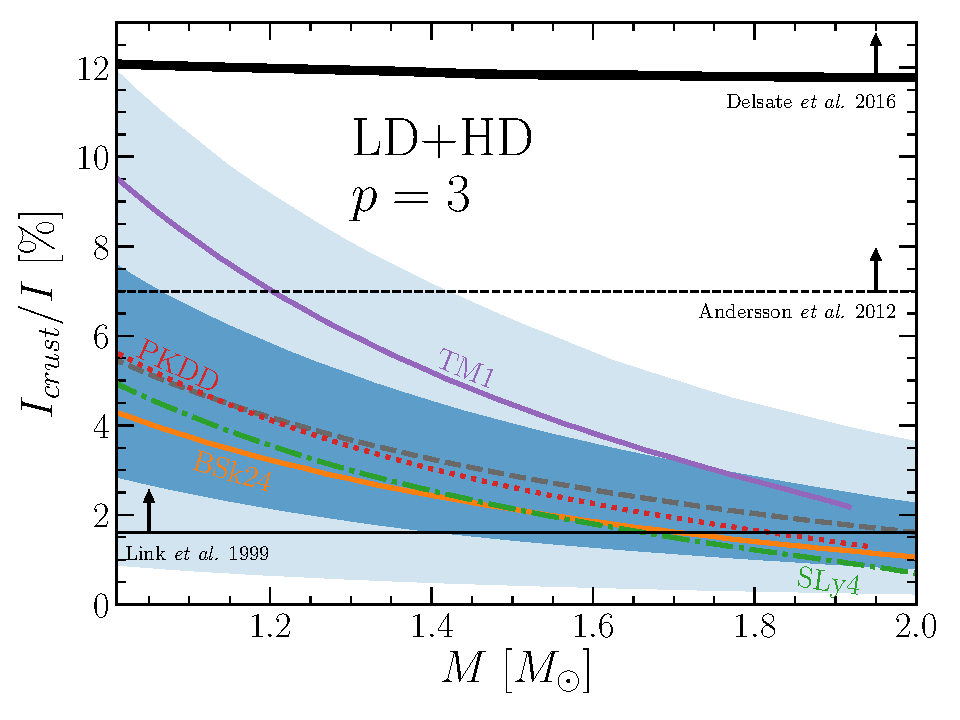
\includegraphics[width=0.9\linewidth]{figures/ifrac_vs_m.pdf}
  \end{center}
  \caption[Marginalized posterior for the fraction of crust moment of inertia
  as a function of the neutron star mass]{Marginalized posterior for the 
    fraction of crust moment of inertia $I_{crust}/I$ as a function of the NS 
    mass $M$, using the LD+HD distribution. The blue dark and light shaded 
    regions show the $50\%$ and $90\%$ confidence intervals, respectively. The 
    gray dashed line represents the average value. 
    The results for four characteristic EoS models are given. 
    The minimum values needed to justify Vela glitches with (Delsate \textit{et
    al.}~\cite{Delsate2016} and Andersson \textit{et al.}~\cite{Andersson2012}) 
    and without (Link \textit{et al.}~\cite{Link1999}) crustal entrainment are 
  represented.}\label{fig:ifrac_vs_m}
\end{figure}

Fig.~\ref{fig:ifrac_vs_m} shows the average value of the fractional crust 
moment of inertia $I_{crust}/I$ and the $50\%$ and $90\%$ regions 
as a function of the NS mass for the LD+HD posterior distribution. It should be
stressed that the uncertainty on $I_{crust}/I$ is smaller 
in~\cite{Carreau2019moi} because this quantity is correlated with the 
isovector empirical parameters $K_{sym}$ and $Q_{sym}$, which are strongly
constrained by the filter on pressure, see Fig.~\ref{fig:iv_dist}, not
accounted for in the present calculation. The black
lines represent the minimum values to justify the large glitches exhibited by
Vela with~\cite{Delsate2016,Andersson2012} and without~\cite{Link1999} 
accounting for the entrainment effect. As expected from~\cite{Link1999}, we
find that the amount of angular momentum stored in the crust is sufficient to
explain pulsar glitches if the entrainment effect is neglected.
Given the intermediate estimation of crustal entrainment~\cite{Andersson2012}
($\langle m_n^*\rangle/m_n = 4.3$), we infer that the mass of Vela must be
lower than $\approx 1.4M_\odot$ to meet the LD+HD prediction at the $90\%$
level. This can also be seen in Fig.~\ref{fig:ifrac14_vs_lcrust14}.
Finally, it is clearly observed that the largest estimation of the crustal 
entrainment effect~\cite{Delsate2016} is incompatible with the present nuclear 
physics knowledge if we keep the standard picture where a full crustal origin 
is assumed~\cite{Anderson1975}. Indeed, it yields $M_\text{Vela} \lesssim 
1M_\odot$, yet such low-mass NS have never been observed to this day. 
%
The same conclusion was drawn in our published paper~\cite{Carreau2019moi}, 
where a different protocol for the fit of the surface energy was employed, and 
a more stringent filter including the chiral EFT pressure estimation was 
included. The fact that the conclusion does not change fully neglecting the EFT 
results on pressure confirms the robustness of the prediction.

\section{Conclusions}\label{sec:conclu2}

In this chapter, we have first introduced the basic equations of hydrostatic 
equilibrium in general relativity, for spherical nonrotating stars. We have
solved these equations for different popular EoS in order to obtain the
relationship between the mass and radius of the star. In the same spirit, we
have computed the moment of inertia as well as the tidal deformability within
the slow rotation approximation, which is expected to be valid for most 
pulsars. The determination of the CC transition density and pressure, discussed
thoroughly in Chapter 1, allows the calculation of crustal observables. We have 
thus computed the crust thickness and fraction of crust moment of inertia. We
have explained in detail the connection between the latter observable and the 
glitch phenomenon in the standard picture, that is where a glitch is observed 
during the transfer of angular momentum from the neutron superfluid in the
inner crust to the rest of the star~\cite{Anderson1975}. 
A major issue exhibited in Section~\ref{sec:tov} is the sensitivity of
the results on the EoS, and more specifically on the isovector empirical
parameters. We have shown that not every EoS successfully pass the maximum mass
constraint of $M_{max} \gtrsim
2M_\odot$~\cite{Demorest2010,Antoniadis2013,Cromartie2020} favoring a stiff 
EoS. 
Moreover, a full crustal origin for the glitch phenomenon can only be accepted 
with very stiff EoS, given the present estimations of crustal 
entrainment~\cite{Andersson2012,Piekarewicz2014}.
Conversely, the recent constraint on the tidal deformability parameter 
$\Lambda_{1.4}$ inferred from GW170817~\cite{GW1} tends to favor soft EoS. 

We have recalled the principle of Bayesian inference before performing the
Bayesian determination of the EoS parameters, using the metamodeling
technique~\cite{Margueron2018a}. We have used a uniform prior distribution for
the parameters, given empirical constraints. 
%
The results and analyses presented in this chapter follow closely, but are not
identical to our published results~\cite{Carreau2019cc,Carreau2019moi}. Indeed,
a Bayesian analysis crucially depends both on the prior and on the choice of
the filters. In the present work, we have varied both the prior distribution of
surface parameters, adopting a different protocol from the one
of~\cite{Carreau2019cc,Carreau2019moi} and introducing curvature terms which
were neglected in the previous study, and the filters, exploring the specific
effect of including or not the EFT predictions of the pressure of SNM and PNM.
The different results are compatible within error bars, but different
correlations are observed. These differences are discussed, and have allowed us
to better understand the effect of the different conditions.
%
A sensitivity analysis on the CC
transition point has revealed that the isovector parameters are 
the most important for the precise determination of $n_t$ and $P_t$.
We have calculated the likelihood function using constraints on nuclear physics
observables (LD constraints), namely the experimental masses~\cite{Huang2017} 
and chiral EFT calculations on SNM and PNM~\cite{Drischler2016}, and on NS
observables as well as physical requirements (HD constraints). The posterior
distribution of empirical parameters was analyzed. We have observed that the
LD filter is very effective in constraining the isovector parameters,
particularly if the impose the compatibility with the chiral ETF predicted
bands for pressure. We have shown that only the constraints arising from
nuclear physics impose correlations among the empirical parameters. In the
isovector sector, the correlation between $E_{sym}$ and $L_{sym}$ is recovered,
and we find that $L_{sym}$ is correlated with $K_{sym}$. We have found
new interesting correlations when imposing pressure filter:
$r(L_{sym},Q_{sym})=-0.55$ and $r(K_{sym},Q_{sym})=0.52$.

Finally, we have made general predictions for the static properties and crustal 
observables of NS, using the LD+HD joint posterior distribution of parameters 
calculated in Section~\ref{sec:bayes}. Overall, we have found that our 
predictions for the NS observables are in a rather good agreement with the
constraints on the EoS, radius, and tidal deformability, inferred from the 
GW170817 event~\cite{De2018,GW1}. We have obtained 
$R_{1.4}=12.88_{-0.65}^{+0.53}$ km and $\Lambda_{1.4} = 634_{-190}^{+204}$ at 
the $90\%$ level. 
We have shown that the transition density and pressure are 
correlated with the isovector parameters, and particularly with the skewness 
parameter $Q_{sym}$. Within the present experimental and theoretical 
uncertainty on those parameters, we have estimated the transition density and
pressure respectively as $n_t=0.068_{-0.021}^{+0.021}$ fm$^{-3}$ and
$P_t=0.263_{-0.149}^{+302}$ MeV/fm$^3$, at the $1\sigma$ confidence level. In
contrast with our previous work~\cite{Carreau2019cc}, with the present protocol 
we do not observe a strong influence of
the surface parameters on the CC transition quantities. This can be explained 
by a refined control of the surface energy in the present work.
We have observed that the thicker the crust is, the more angular momentum is
confined to the neutron superfluid coexisting with the crystal lattice in the
inner crust. The large uncertainty on the transition pressure is reflected on
the fraction of crust moment of inertia. Indeed, for a $1.4M_\odot$ NS, we have 
obtained $I_{crust,1.4}/I_{1.4}=2.89_{-1.68}^{+2.51} \%$, at the $1\sigma$ 
confidence level. The joint distribution for Vela mass and radius was
computed for two different estimations of the crustal entrainment effect. It 
has confirmed that a control on crustal entrainment is the key phenomenon to
associate the glitch phenomenon to crustal physics, even if the uncertainty on
the EoS blurs the results. We have observed the variation with NS
mass of the fraction of crust moment and inertia and concluded that a full 
crustal origin is excluded if we consider the present largest estimation of 
crustal entrainment~\cite{Delsate2016}.

\clearpage\thispagestyle{empty}
